\documentclass[12pt,a4paper,bibliography=totocnumbered,listof=totocnumbered]{scrartcl}
\usepackage[ngerman]{babel}
\usepackage[utf8]{inputenc}
\usepackage{amsmath}
\usepackage{amsfonts}
\usepackage{amssymb}
\usepackage{graphicx}
\usepackage{fancyhdr}
\usepackage{tabularx}
\usepackage{geometry}
\usepackage{setspace}
\usepackage[right]{eurosym}
\usepackage[printonlyused]{acronym}
\usepackage{subfig}
\usepackage{floatflt}
\usepackage[usenames,dvipsnames]{color}
\usepackage{colortbl}
\usepackage{paralist}
\usepackage{array}
\usepackage{titlesec}
\usepackage{parskip}
\usepackage[right]{eurosym}
\usepackage{picins}
\usepackage[subfigure,titles]{tocloft}
\usepackage[pdfpagelabels=true]{hyperref}
\usepackage{listings}

\usepackage{color}

% \lstset{basicstyle=\footnotesize, captionpos=b, breaklines=true, showstringspaces=false, tabsize=2, frame=lines, numbers=left, numberstyle=\tiny, xleftmargin=2em, framexleftmargin=2em}
% \makeatletter
% \def\l@lstlisting#1#2{\@dottedtocline{1}{0em}{1em}{\hspace{1,5em} Lst. #1}{#2}}
% \makeatother

\geometry{a4paper, top=27mm, left=30mm, right=20mm, bottom=35mm, headsep=10mm, footskip=12mm}

% \hypersetup{unicode=false, pdftoolbar=true, pdfmenubar=true, pdffitwindow=false, pdfstartview={FitH},
% 	pdftitle={Abschlussarbeit},
% 	pdfauthor={Daniel Brettschneider},
% 	pdfsubject={Abschlussarbeit},
% 	pdfcreator={\LaTeX\ with package \flqq hyperref\frqq},
% 	pdfproducer={pdfTeX \the\pdftexversion.\pdftexrevision},
% 	pdfkeywords={Abschlussarbeit},
% 	pdfnewwindow=true,
% 	colorlinks=true,linkcolor=black,citecolor=black,filecolor=magenta,urlcolor=black}
% \pdfinfo{/CreationDate (D:20110620133321)}

\begin{document}

\titlespacing{\section}{0pt}{12pt plus 4pt minus 2pt}{-6pt plus 2pt minus 2pt}

% Kopf- und Fusszeile
\renewcommand{\sectionmark}[1]{\markright{#1}}
\renewcommand{\leftmark}{\rightmark}
\pagestyle{fancy}
% \chead{}
% \cfoot{}
\renewcommand{\headrulewidth}{0.4pt}
\renewcommand{\footrulewidth}{0.4pt}

% Vorspann
\renewcommand{\thesection}{\arabic{section}}
\renewcommand{\theHsection}{\arabic{section}}
% default page numbering
% \pagenumbering{arabic}

% ----------------------------------------------------------------------------------------------------------
% Titelseite
% ----------------------------------------------------------------------------------------------------------
\thispagestyle{empty}
\begin{center}
	
\includegraphics[scale=1]{Bilder/uni_os_l.png}\\
	\vspace*{2cm}
	\Large
	\textbf{Fachbereich}\\
	\textbf{Humanwissenschaften}\\
	\textbf{Institut für Cognitive Science}\\
	\vspace*{2cm}
	\Huge
	\textbf{Bachelorarbeit}\\
	\vspace*{0.5cm}
	\large
	Automatisierte Analyse von Preisbildungsmustern\\
	anhand von Zeitreihendaten der Markttransparenzstelle für Kraftstoffe\\
	% \vspace*{1cm}
	% \textbf{Ausblick}\\
	\vspace*{2cm}
	
	\vfill
	\normalsize
	\newcolumntype{x}[1]{>{\raggedleft\arraybackslash\hspace{0pt}}p{#1}}
	\begin{tabular}{x{6cm}p{7.5cm}}
		\rule{0mm}{5ex}\textbf{Autor:} & Kai Fritsch\newline kai.m.fritsch@gmail.com \\ 
		\rule{0mm}{5ex}\textbf{Prüfer:} & Prof. Dr. Oliver Vornberger \\ 
		% \rule{0mm}{5ex}\textbf{Abgabedatum:} & - \\ 
	\end{tabular} 
\end{center}
\pagebreak

% ----------------------------------------------------------------------------------------------------------
% Verzeichnisse
% ----------------------------------------------------------------------------------------------------------
% TODO Typ vor Nummer
% \renewcommand{\cfttabpresnum}{Tab. }
% \renewcommand{\cftfigpresnum}{Abb. }
% \settowidth{\cfttabnumwidth}{Abb. 10\quad}
% \settowidth{\cftfignumwidth}{Abb. 10\quad}

% \titlespacing{\section}{0pt}{12pt plus 4pt minus 2pt}{2pt plus 2pt minus 2pt}
% \singlespacing
% \rhead{INHALTSVERZEICHNIS}
% \renewcommand{\contentsname}{II Inhaltsverzeichnis}
% \phantomsection
% \addcontentsline{toc}{section}{\texorpdfstring{II \hspace{0.35em}Inhaltsverzeichnis}{Inhaltsverzeichnis}}
% \addtocounter{section}{1}
% \lhead{Inhaltsverzeichnis}
\tableofcontents
\pagebreak
% \rhead{VERZEICHNISSE}
% \listoffigures
% \pagebreak
% \listoftables
% %\pagebreak
% \renewcommand{\lstlistlistingname}{Listing-Verzeichnis}
% {\labelsep2cm\lstlistoflistings}
% \pagebreak

% ----------------------------------------------------------------------------------------------------------
% Abkürzungen
% ----------------------------------------------------------------------------------------------------------
% \section{Abkürzungsverzeichnis}
% \begin{acronym}[OSGi] % längste Abkürzung steht in eckigen Klammern
% 	\setlength{\itemsep}{-\parsep} % geringerer Zeilenabstand
% 	\acro{OSGi}{Open Service Gateway initiative}
% \end{acronym}
% \newpage

% ----------------------------------------------------------------------------------------------------------
% Abstract
% ----------------------------------------------------------------------------------------------------------

% Seitenzähler starten
\setcounter{page}{1}
\rfoot{\ \linebreak Seite \thepage}
% Zeilenabstand setzen
\onehalfspacing
\rhead{\thesection\space\contentsname}
% own page numbering

% ----------------------------------------------------------------------------------------------------------
% Einleitung
% ----------------------------------------------------------------------------------------------------------
\titlespacing{\section}{0pt}{12pt plus 4pt minus 2pt}{2pt plus 2pt minus 2pt}
\lhead{Einleitung}
\section{Einleitung}

\titlespacing{\subsection}{0pt}{12pt plus 4pt minus 2pt}{-6pt plus 2pt minus 2pt}
\subsection{Geschichtlicher Hintergrund}
Kraftstoffpreise unterliegen nun schon seit längerer Zeit großen Preisschwankungen. Die hohe Homogenität und sinkende Nachfrage sind optimale Bedingungen für starken Konkurrenzdruck. Der Druck ist so hoch, dass die Anzahl an Tankstellen in Deutschland seit 1970 von gut 46.000 auf heute knapp 15.000 gefallen ist.\cite{PraTa} Nichts desto trotz ist die Anzahl an Preisänderungen in den letzten Jahren noch einmal merklich gestiegen. Während der Preis 2011 noch durchschnittlich weniger als zwei mal pro Tag geändert wurde, sind die meisten Tankstellen inzwischen bei um die sechs Änderungen pro Tag angelangt.\cite{Unity} \\

%TODO: Check for Pricings per Day for each month since start\\

Mitgrund für diese jüngste Steigerung könnten diesmal jedoch die neuerlichen elektronischen Möglichkeiten sein. Während Tankstelleninhaber vor einigen Jahren noch ihrer Konkurrenz einen Besuch abstatten mussten um deren Preise auszukundschaften, reicht heute eine Suchanfrage im Internet. Und selbst diese ist seit der Einführung der Markttransparenzstelle für Kraftstoffe nicht mehr notwendig. Jede Tankstelle ist seit Ende 2013 verpflichtet ihre Preisänderungen dem Bundeskartelamt für Kraftsotffe elektronisch zu übermitteln. Der auf diese Weise enstandene Datensatz  bildet die Grundlagen dieser Arbeit.\\

\titlespacing{\subsection}{0pt}{12pt plus 4pt minus 2pt}{-6pt plus 2pt minus 2pt}
\subsection{Pricing Strategien}
Tankstellen waren in den letzten Jahren immer wieder gezwungen ihre Strategien dem immer schneller werdenden Markt anzupassen. Die mit der neuerlichen Änderung verbundene zentrale und unmittelbare Verfügbarkeit aller aktuellen Preise ermöglicht es Tankstellenbesitzern ihre Preise innerhalb kürzester Zeit an die Konkurrenz anzupassen. Das bestehen einer einheitlich definierten Schnittstelle ermöglicht es auch Preisänderungen zunächst automatisch zu registrieren und anschließend sogar die diesbezüglich relevanten eigenen Preise anhand von Regeln ebenfalls automatisch anpassen zu lassen. So eine Automatisierung birgt aber auch Probleme.\\
Die Vereinfachung der Arbeit durch automatische Prozesse führt auch dazu, dass mehr Konkurrenten bei gleichzeitig geringerem Aufwand überwacht werden können und die jeweilig gewünschten Reaktionen viel zuverlässiger durchgeführt werden können. Somit steigt aber auch die generelle Anzahl der Preissenkungen und damit auch die eigenen Preise. Um dem entgegen zu wirken müssen die Preise zu Anfang des Tages höher angesetzt werden. Inzwischen wurde sogar eine Mittagserhöhung eingeführt um dem Preisverfall entgegen zu wirken.Auch eine gewisse Abstimmung von Preisen zwischen den Konkurrenten wird immer wichtiger. Wollen zwei Tankstellen jeweils einen günstigeren Preis fahren als die jeweils andere, so würde der Preis kontinuierlich sinken, bis eine Tankstelle ihr Minimum erreicht hat. Es gibt unter Tankstellen deshalb so etwas, wie eine Rangordnung, die den Markt in A-Preiser und B-Preiser unterteilt. A-Preiser, zumeist die Markentankstellen, erlauben den B-Preisern, zumeist freie Tankstellen oder kleinere Ketten, etwas geringer Preise zu fahren. Während der Preisverfall bei einem Verstoß gegen diese Rangordnung vor der Automatiserung noch relativ langsam von statten ging, liegt der Preis bei automatischem Pricing innerhalb weniger Minuten beim Minimum. Zudem muss jegliche Art von Sonderfällen in den Regeln berücksichtigt werden. Um ungewünschten Preisen durch einen vollautomatischen Betrieb vorzubeugen beschränkt sich die Automatisierung teilweise auf den Vorschlag von Preisänderungen, welche dann noch manuell durchgeführt werden müssen.\\
% Interview mit Jonathan!!!!!!!!!!!!!!!!

\titlespacing{\subsection}{0pt}{12pt plus 4pt minus 2pt}{-6pt plus 2pt minus 2pt}
\subsection{Motivation}
Die Idee dieser Arbeit besteht darin das Konkurrenzverhalten der Tankstellen zu analysieren. Es ist anzunehmen, dass eine Tankstelle egal ob manuel oder automatisch ihr Preise nicht zufällig anpasst, sondern versucht sie möglichst gewinnoptimierend zu gestalten. Preise sollten also generell nach bestimmten Richtlinien in Abhängigkeit von verschiedenen Parametern festgelegt werden. Wo konsistent nach bestimmten Parametern Entscheidungen getroffen werden, entstehen Regeln, die auch zurückverfolgt werden können. Je konsistenter eine Regel umgesetzt wird, desto einfacher ist es diese anhand ihrer Auswirkungen zu rekonstruieren. Je automatisierter also eine Tankstelle ihr Pricing betreiben, desto einfacher sollte es sein ihr Verhalten zu analysieren.\\

\titlespacing{\subsubsection}{0pt}{12pt plus 4pt minus 2pt}{-6pt plus 2pt minus 2pt}
\subsubsection{Unmittelbar Nutzen}
In einem Wettbewerb ist es immer von Vorteil die Strategien der Konkurrenten zu kennen. Es ermöglich eine akkuratere Vorhersage des zukünftigen Verlaufes und erlaubt es einem somit seine eigene Strategie gewinnbringender zu gestalten. Da das Pricing in großen Ketten zentral betrieben wird, liegt die Verantwortung über das Preisverhalten von mehreren Hunderten Tanstellen bei einem sehr kleinen Personenkreis. Bei beispielsweise 100 Tankstellen mit jeweils fünf potentiellen Konkurrenten und sechs Preisänderungen pro Tag müssten diese Personen Regeln für 500 Konkurrenten in 3000 Preisänderugnen täglich erkennen. Eine automatisierte Regelerkennung würde also viel Arbeit und Mühen ersparen und wahrscheinlich sogar verlässlichere Ergebnisse liefern. Die eingesparte Zeit kann also in die Optimierung des eingenen Verhaltens investiert werden und die verlässlicheren Ergebnisse liefern eine bessere Grundlage für gezielte Optimierungen.\\

\titlespacing{\subsubsection}{0pt}{12pt plus 4pt minus 2pt}{-6pt plus 2pt minus 2pt}
\subsubsection{Potentielle Möglichkeiten}
Jede Preissenkung verringert die Gewinnspanne einer Tankstelle. Es liegt also prinzipiell nicht im Interesse einer Tankstelle Preise zu senken. Angenommen eine automatisierte Regelerkennung wäre gegeben. Es bestehen einige Möglíchkeiten dieses Wissen gewinnbringend zu nutzen:
\begin{itemize}
\item Mit einer solchen Regelerkennung ließen sich reaktive Preisänderungen von aktiven unterscheiden. Einzelne Änderungen könnten somit iterativ über die jeweiligen auslösenden Konkurrenten zurückverfolgt werden bis hin zu einer aktiven Änderung, also dem eigentlichen Auslöser. Die Erkennung von Auslösern bietet dann Möglichkeiten andersweitig zu reagieren und Senkungen zu umgehen.
\item Ebenso denkbar wäre, dass es diese Auslöser in Form von aktiven Senkungen gar nicht so häufig gibt. Angenommen Tanstellen würden zwar bei Senkungen aufeinander reagieren, ihre Erhöhungen aber unabhängig gestalten. Eine Tankstelle die Ihre Preise weniger hoch erhöht wäre somit potentieller Auslöser von einer Senkungswelle. Es wäre also unter Umständen möglich, dass man sich intensiver mit den eigenen Erhöhungen beschäftigen müsste.
\item Es ist bereits ohne dieses Tool möglich einige Preisänderungen über größere Strecken zurückzuverfolgen. Mit dem Tool bestünde die Möglichkeit Verkettungen von Konkurrenten zu erkennen und diese Wege exakt aufzuzeigen. Man könnte dann versuchen diese Ketten zu unterbrechen, sodass isoliertere Preissektoren entstünden.
\item Es bietet auch die Möglichkeit die eigenen Änderungen systematisch zu analysierenund und weniger wichtige Konkurrenten aus dem System zu nehmen.
\end{itemize}
Diese Änderungen müssen jedoch nicht zwangsläufig nur den Tankstellen zu Gute kommen. Eine Tankstelle ist gesetzlich verpflichtet keine verlustbringenden Preise zu fahren um Preisdumping zu vermeiden. Sie muss somit die ganzen Preissenkungen an einem Tag in die Preiserhöhung zu Tagesbeginn einkalkulieren. Das ist höchstwahrscheinlich auch ein Grund für die erst kürzlich eingeführte Mittagserhöhung. Eine Verminderung der Preissenkungen führt somit nicht zwangsweise zu höheren Preisen, da weiterhin ein Wettbewerb besteht. Es sollte vielmehr zu generell stabileren Preisen führen, sodass Kunden sich besser auf Preise verlassen können.

\newpage
\vspace{-1,2em}
% ----------------------------------------------------------------------------------------------------------
% Grundlagen
% ----------------------------------------------------------------------------------------------------------
\lhead{Grundlagen}
\titlespacing{\section}{0pt}{12pt plus 4pt minus 2pt}{-6pt plus 2pt minus 2pt}
\section{Grundlagen}
Dieses Kapitel soll einen Überblick über die mir zur Verfügung stehenden Informationen, sowie die von mir verwendeten Tools liefern. 
Zu den Informationen zählen zum Einen der Datensatz der Markttransarenzstelle(MTS) für Kraftstoffe, sowie zum Anderen der exemplarische Aufbau eines der auf dem Markt verfügbaren automatischen Pricing-Tools. Zusätzlich dazu habe ich noch einen groben Erfahrungsbericht, wie dieses Tool bei einer Tankstelle eingesetzt wird.

\titlespacing{\subsection}{0pt}{12pt plus 4pt minus 2pt}{-6pt plus 2pt minus 2pt}
\subsection{Datensatz}

\begin{quote} 
\glqq Seit dem 31. August 2013 sind Unternehmen, die öffentliche Tankstellen betreiben oder über die Preissetzungshoheit an diesen verfügen, verpflichtet, Preisänderungen bei den gängigen Kraftstoffsorten Super E5, Super E10 und Diesel in Echtzeit an die Markttransparenzstelle für Kraftstoffe zu melden.\grqq\cite{BkMTS}
\end{quote}

In Echtzeit bedeutet, dass die Information über eine Preisänderung spätestens 5 Minuten nach der Änderung selber an der MTS eingehen müssen. Neben den Preisänderungen müssen auch die Stammdaten der Tankstellen wöchentlich an die MTS gemeldet werden. Die MTS veröffentlicht die Daten nicht direkt selber, sondern stellt sie Verbraucherinformationsdiensten(VID) zur Verfügung. Diese verpflichten sich die Daten in irgendeiner den Verbrauchern nützlichen Form zu veröffentlichen. Die Schnittstelle der MTS ist in der folgenden Abbildung dargestellt.

% \begin{center}
% 	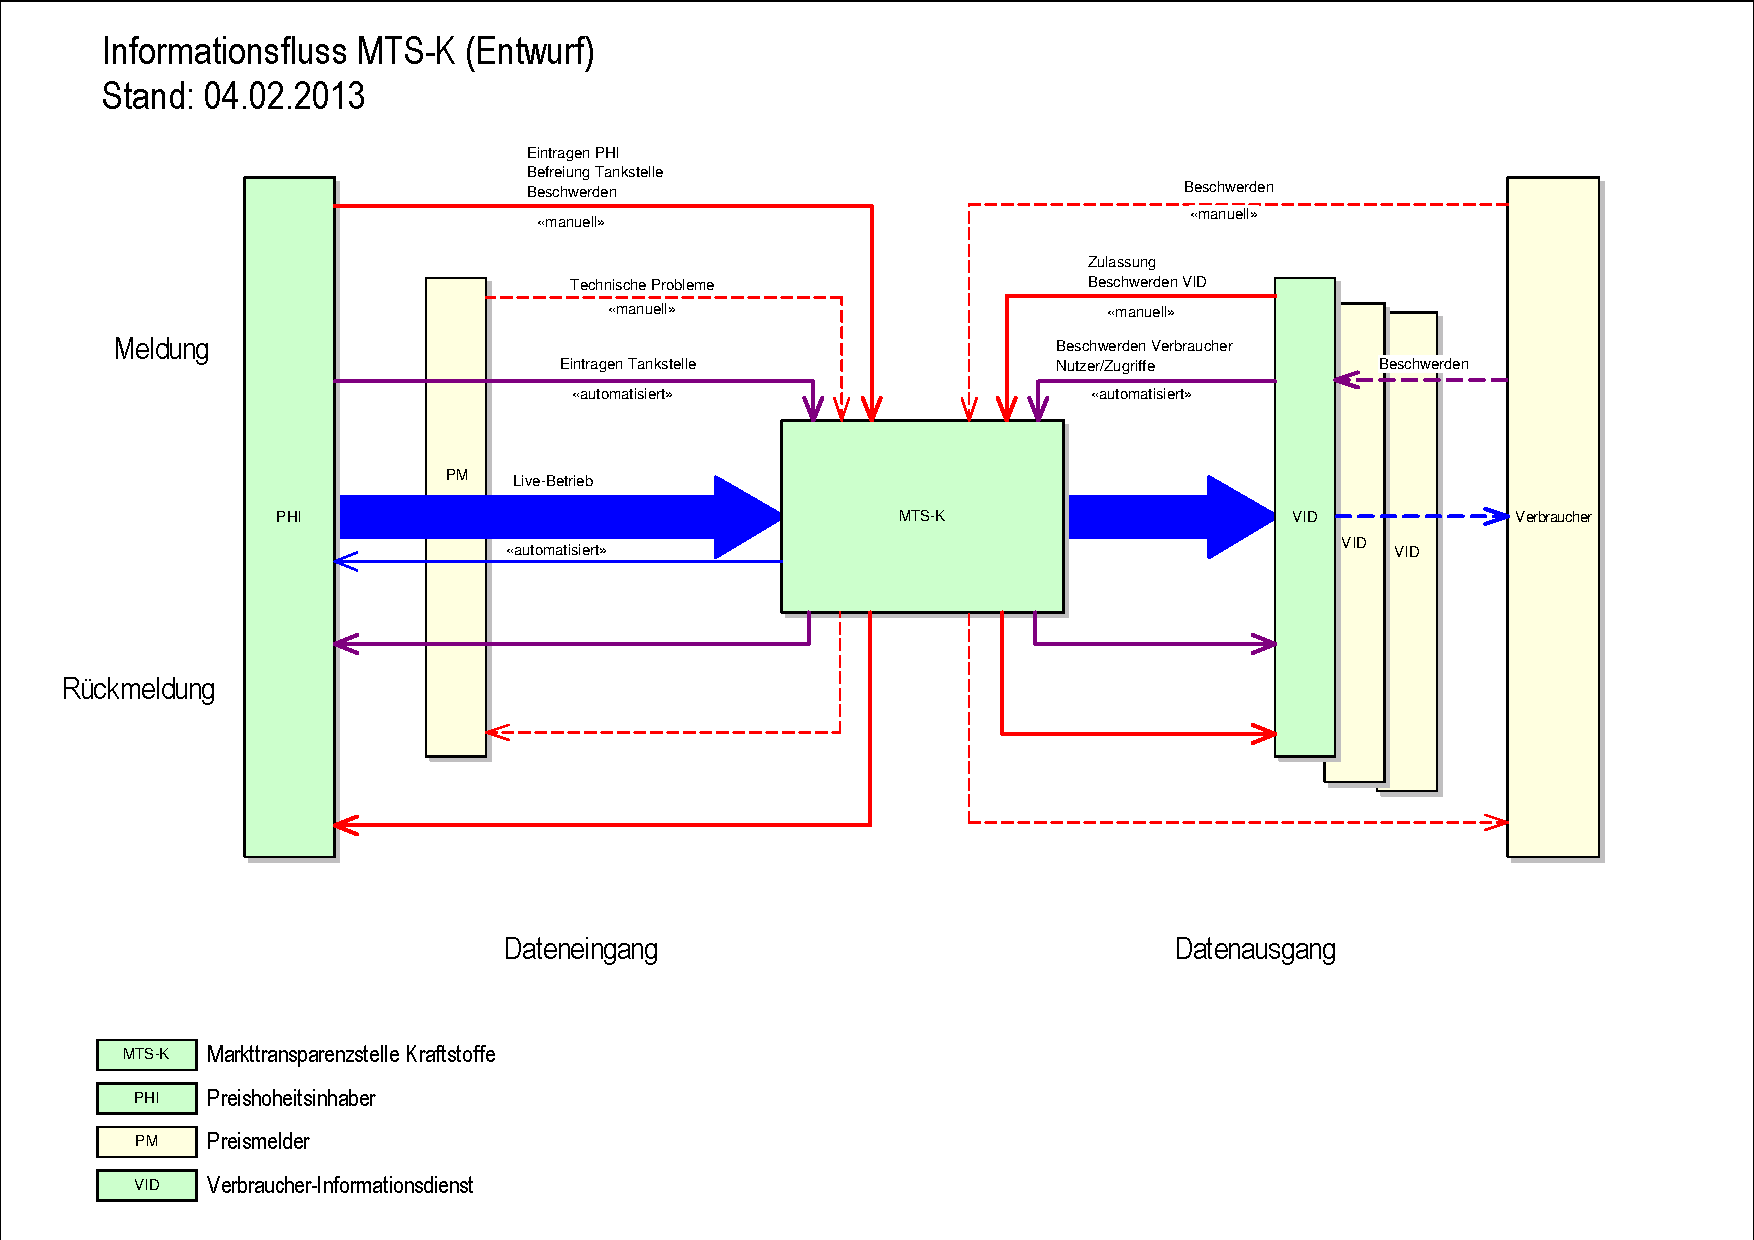
\includegraphics[width=0.8\textwidth]{Bilder/Informationsfluss-MTS.png}\\
% 	\captionof{figure}[IMTS]{Informationsfluss der MTS-K\cite{IMTSK}}
% 	\label{fig:MTS-K}
% \end{center}

\begin{center}
	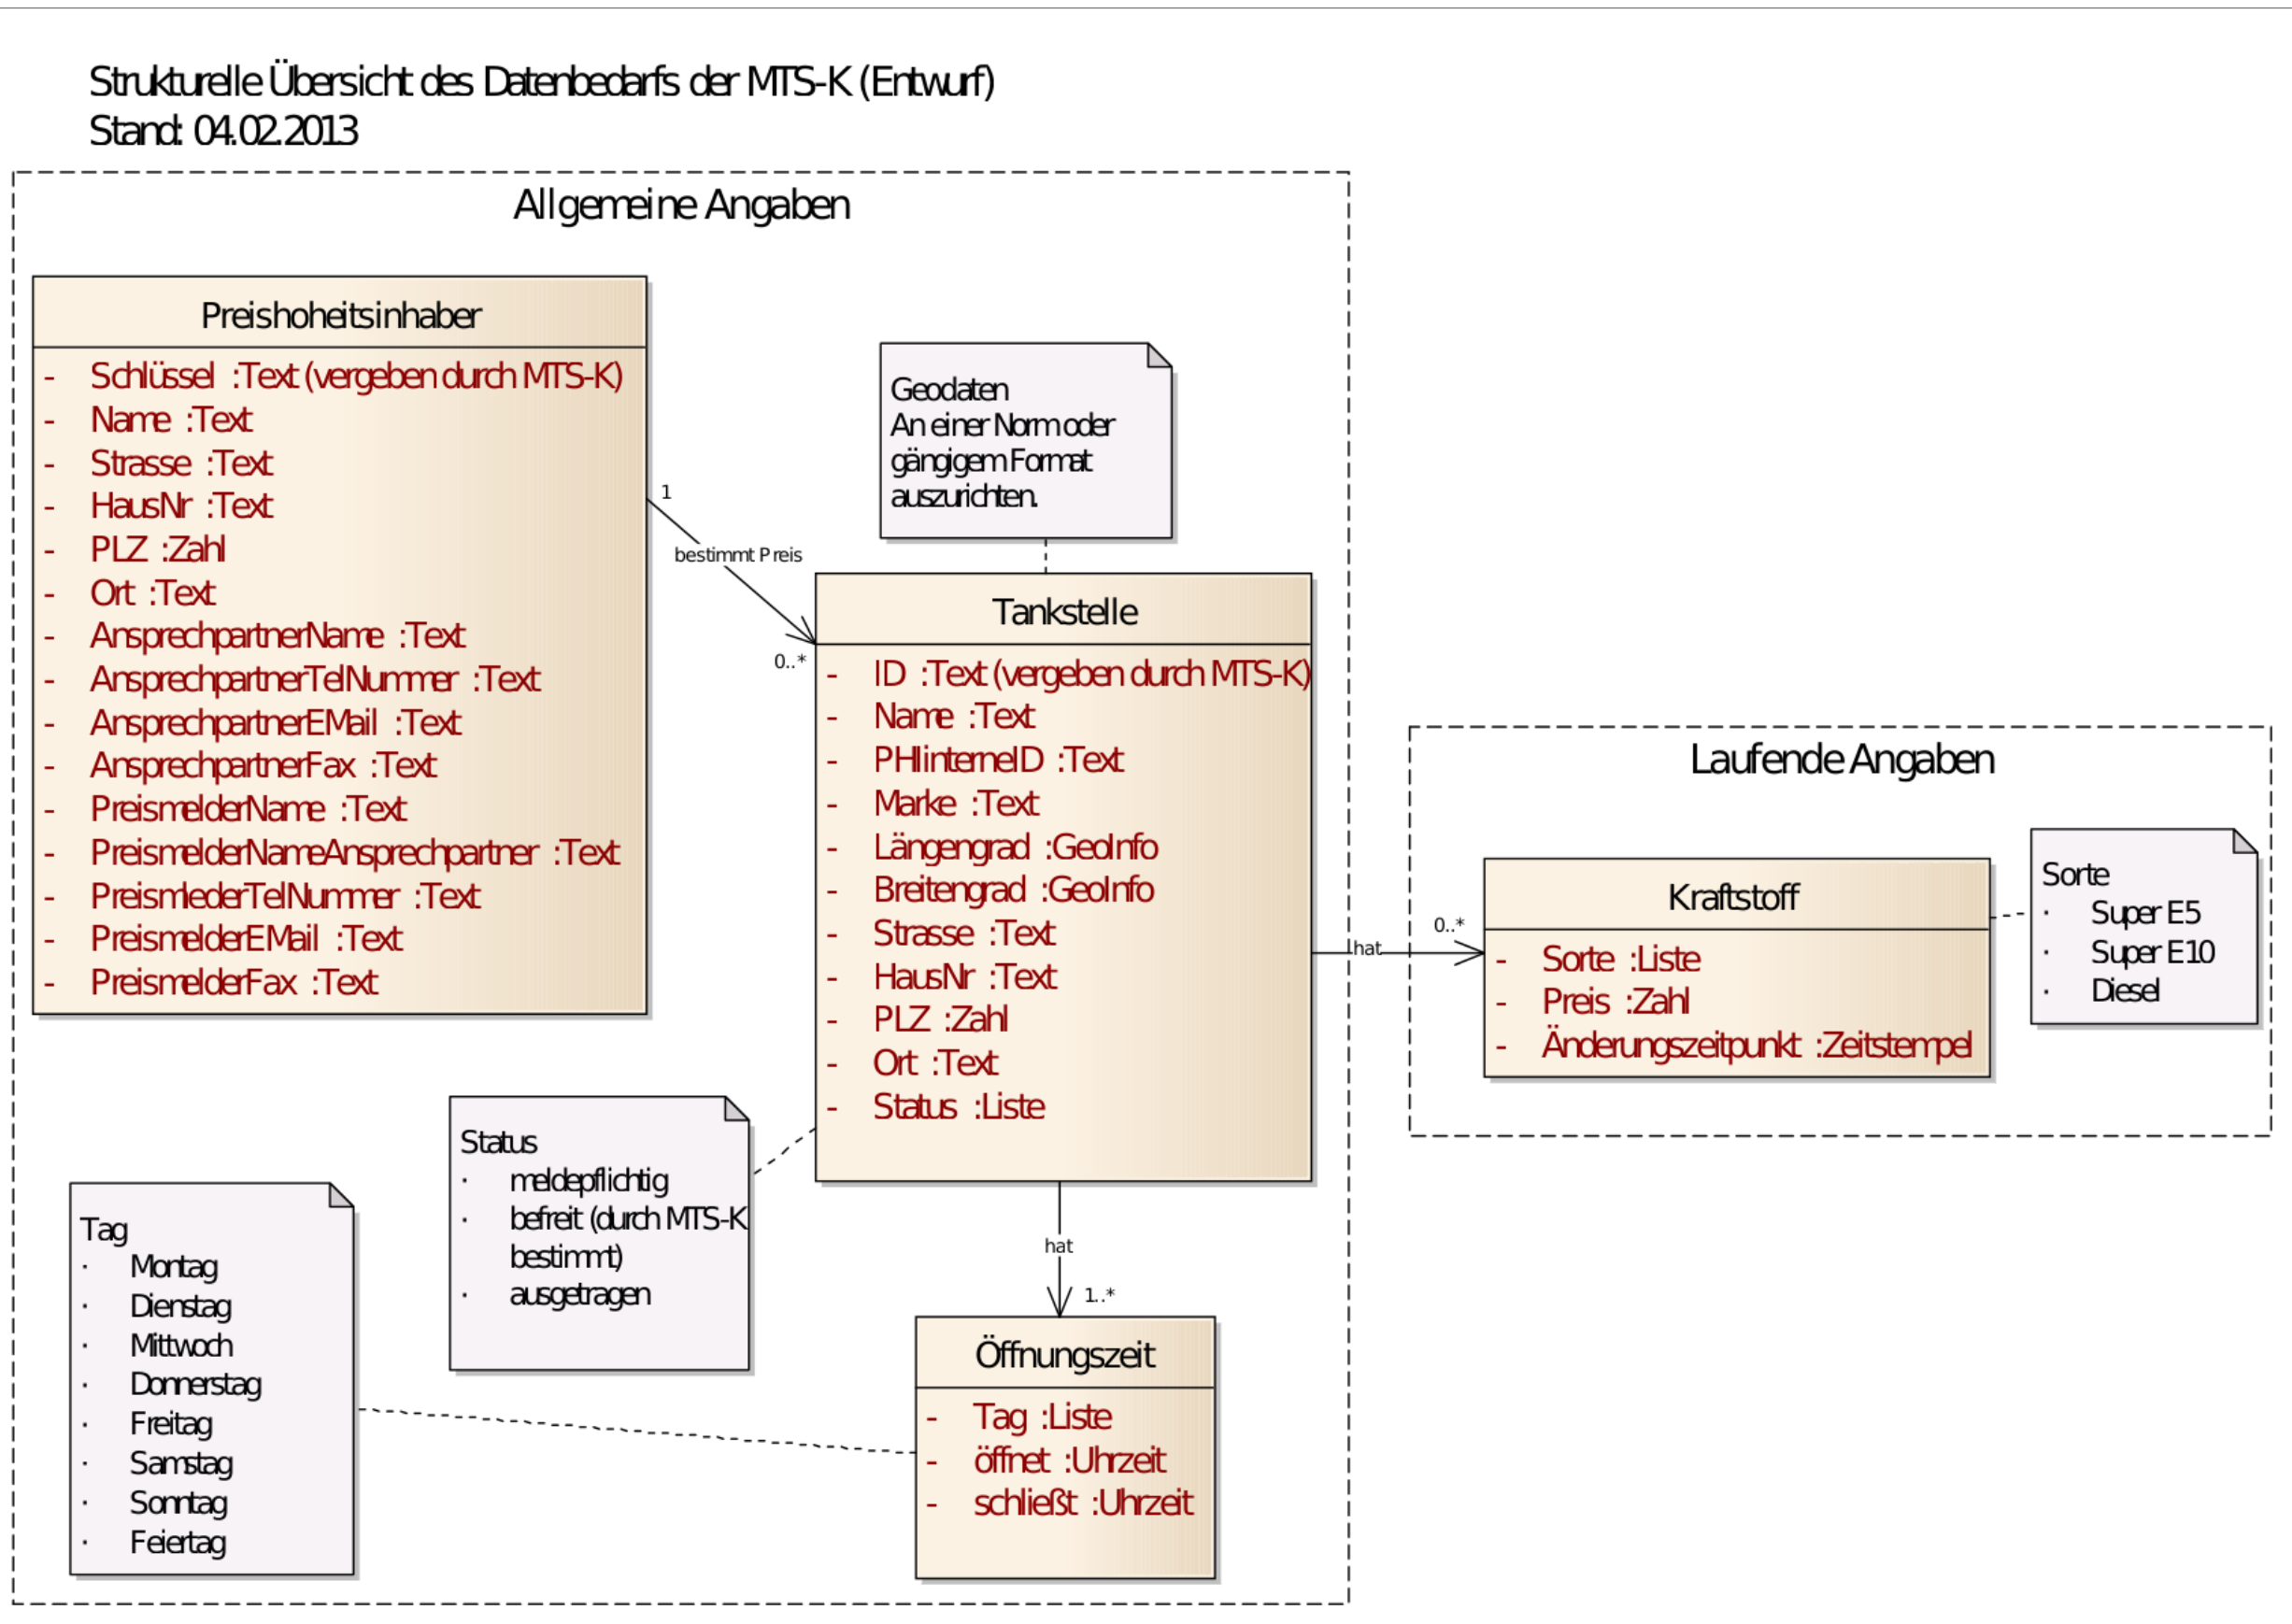
\includegraphics[width=0.8\textwidth]{Bilder/Datenstruktur-MTS.png}\\
	\captionof{figure}[DMTS]{Datenstruktur der MTS-K\cite{DMTSK}}
	\label{fig:MTS-K}
\end{center}

Die Daten für diese Arbeit entstammen dem Verbraucherinformationsdienst der Tankerkönig API. Tankerkönig bezieht seine Daten direkt von der MTS  und stellt diese sowohl im Zuge einer Echtzeit-Benzinpreis-API als auch gesondert aufbereitet als historischen Datenbank in Form eines PostgreSQL dumps im 9.4.-Format zur Verfügung. Die für diese Arbeit verwendeten dumps umfassen neben den kompletten Preisdaten vom 8.6.2014 bis heute auch die Informationen über die Stammdaten der Tankstellen.\cite{TkAPI} 

\begin{center}
	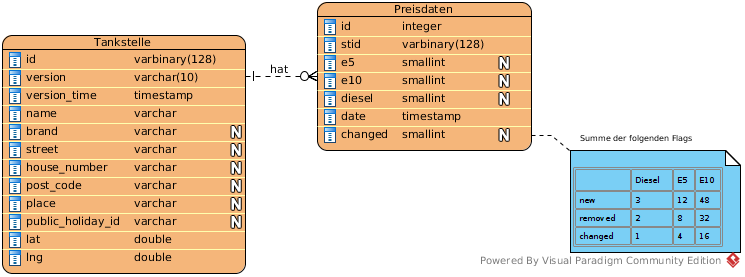
\includegraphics[width=0.8\textwidth]{Bilder/pricing_data.png}\\
	\captionof{figure}[ERD Tankerkönig]{ERD des historischen Datensatzes}
	\label{fig:ERD-T}
\end{center}

Alle für diese Arbeit verfügbaren Informationen sind in der Abb.2 abgebildet. Die Daten aus dem MTS-Datensatz werden größtenteils von den Tankstellen selber zur Verfügung gestellt, weshalb die Felder teilweise nicht einheitlich definiert sind. Die id wird als einziges von der MTS bereitgestellt. Die Felder \textit{$version_timestamp$} and \textit{version} wurden dem Datensatz von Tankerkönig hinzugefügt und identifizieren wann Änderungen an den Stammdaten einer Tankstelle vorgenommen wurden, beziehungsweise zählen die verschiedenen Versionen. Die Felder \textit{name} und \textit{brand} werden von den Tankstellen selber befüllt und enhalten sehr verschiedene Informationen. Bei großen Markentankstellen wird unter \textit{brand} die Marke geführt und als \textit{name} wird hier oft schon die Adresse aufgeführt, da diese offenbar als Identifizierung innerhalb des Unternehmens dient. Einzelne Tankstellen oder kleinere Unternehmen machen zu \textit{brand} entweder keine Angaben oder irgendwie auf andere weise kenntlich, dass sie keinem großen Konzern angehören. Bei \textit{name} geben Sie dann meistens den Inhaber oder den Unternehmensnamen an. Bei den Feldern zur Adresse fehlen teilweise Informationen oder sie werden zusammen aufgeführt. Beispielsweise taucht die Hausnummer des öftern schon im Straßenfeld mit auf. Der public holiday identifier gibt an welchem Bundesland dieser Standort angehört und damit die entsprechend geltenden Feier- und Ferientage. Der Standort kann über lat und lng eindeutig identifiziert werden.\\
Bei den Preisänderungen hat Tankerkönig die neu angeschlagenen Preise der Kraftstoffsorten Diesel, E5 und E10, den Identifier der Tankstelle \textit{stid}, und den Zeitstempel \textit{date} übernommen. Zudem wurde unter \textit{id} ein Zähler über alle Änderungen, sowie mit \textit{changed} ein Identifier für die geänderten Kraftstoffsorten, hinzugefügt. Diese Identifier errechnet sich aus der Summe der entsprechenden Felder der kleinen Tabelle und gibt nicht nur an ob ein Preis geändert wurde, sondern auch, ob dieser auf Null gesetzt (removed), oder von Null wieder erhöht (new) wurde.\\

\titlespacing{\subsection}{0pt}{12pt plus 4pt minus 2pt}{-6pt plus 2pt minus 2pt}
\subsection{PSQL Datenbank}

\titlespacing{\subsubsection}{0pt}{12pt plus 4pt minus 2pt}{-6pt plus 2pt minus 2pt}
\subsubsection{Funktion}

\titlespacing{\subsubsection}{0pt}{12pt plus 4pt minus 2pt}{-6pt plus 2pt minus 2pt}
\subsubsection{Indexing}

\titlespacing{\subsection}{0pt}{12pt plus 4pt minus 2pt}{-6pt plus 2pt minus 2pt}
\subsection{Verwendete Programme und Packages}

\titlespacing{\subsection}{0pt}{12pt plus 4pt minus 2pt}{-6pt plus 2pt minus 2pt}
\subsection{Pricing-Tool}

Neben den Verbraucher kommen diese Informationen auch den Tankstellenbesitzern zu Gute. Die einheitlich definierte technische Informationsschnittstelle ermöglicht es Preise automatisch ohne Zeitverzögerung anzupassen. Die Homogenität des Produktes, der für den Kunden einzig interessante Unterschied im Bezug auf das Produkt ist der Preis selber, sorgt gleichzeitig dafür, dass Preisanpassungregeln eine relativ einfache Struktur aufweisen können. Aufgrund dieser Simplizität, sind in den letzten Jahren einige Pricing-Tools enstanden die das Pricingverhalten zumindest teilweise automatisieren. Während mittelständische Unternehmen auf externe Software Lösungen zurückgreifen, so wie zum Beispiel die Q1 und Westfalen AG auf Angebote der Firmen Temiz4u\footnotemark[1] und Weat\footnotemark[2], ist anzunehmen, dass zumindest die größten fünf Mineralölkonzerne Deutschlands, Aral, Shell, Jet, Esso und Total, intern entwickelte Programme verwenden dürften. Im folgenden werden am Beispiel eines Tools die Einstellungsmöglichkeiten für den  Nutzer erklärt, die diesem bei der Definition seiner Regeln zur Verfügung stehen. Diese Optionen stellen gleichsam die Parameter dar, die im Zuge dieser Arbeit aus dem Datensatz extrahiert werden sollen.

\footnotetext[1]{Quelle: \url{https://www.temiz4u.net/web/guest/solutions}}
\footnotetext[2]{Quelle: \url{http://www.weat.de/produkte/pricing/}}

\titlespacing{\subsubsection}{0pt}{12pt plus 4pt minus 2pt}{-6pt plus 2pt minus 2pt}
\subsubsection{Funktionsweise}
Im folgenden werden die für diese Arbeit relevanten Funktionen eines solchen Tools beschrieben. Es wird für diese Arbeit angenommen das andere Tools inhaltlich ähnlich funktionieren. Das hier vorgestellte Tool erhält über einen oder mehrere Verbraucherinformationsdienst die aktuellen Preisänderungen aller Tankstellen. Beim eintreffen einer Änderung wird überprüft, ob diese Änderung eine von dem Nutzer hinterlegte Regel verletzt. Wird eine Regel verletzt wird darauf in der wiederum vom Nutzer gewählten Art und Weise reagiert. Die Nutzereinstellungen lassen sich in die drei Teilaspekte, Konkurrenten bestimmen, Regel festlegen und Automatisierungsgrad wählen gliedern. 

\titlespacing{\subsubsection}{0pt}{12pt plus 4pt minus 2pt}{-6pt plus 2pt minus 2pt}
\subsubsection{Konkurrenz bestimmen}
\begin{center}
	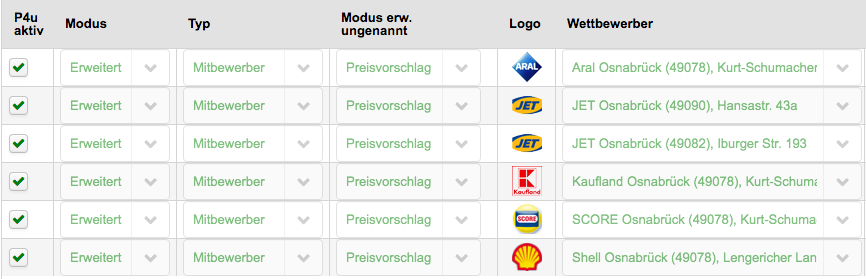
\includegraphics[width=0.8\textwidth]{Bilder/konkurenz.png}\\
	\captionof{figure}[PT-K]{Princing Tool Konkurrenz Bestimmung}
	\label{fig:PT-K}
\end{center}
Hier wird eine Liste von Tankstellen zusammengestellt, die als Konkurrenten erachtet werden. Diese Liste dient als erster Filter für die einkommenden Änderungen. Es werden im weiteren nur Änderungen überprüft, deren Tankstelle in dieser Liste vorzufinde ist.

\titlespacing{\subsubsection}{0pt}{12pt plus 4pt minus 2pt}{-6pt plus 2pt minus 2pt}
\subsubsection{Regeln festlegen}
\begin{center}
	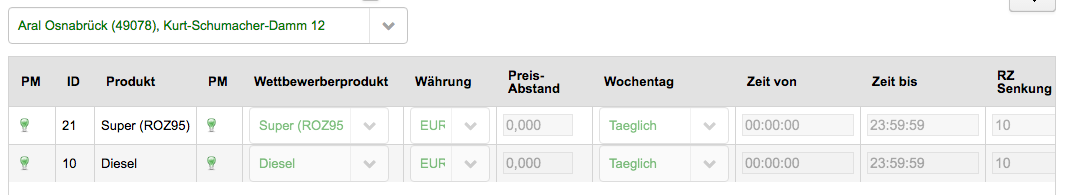
\includegraphics[width=0.8\textwidth]{Bilder/regeln1.png}\\
	\captionof{figure}[PT-R]{Princing Tool Regel Festlegung}
	\label{fig:PT-R}
\end{center}
Für jeden Konkurenten kann ein eigenes Regelwerk angelegt werden. Jede Regel legt zunächst einen untersten Preisabstand für eine bestimmte Spritsorte fest, welcher zu dem jeweiligen Konkurrenten bewahrt werden soll. Positive Werte besagen, dass die Tankstelle selber maximal um den genannten Betrag teuerer sein will als der entsprechende Konkurrent. Negative Werte besagen dementsprechend, dass die Tanstellen selber mindestens um diesen Betrag günstiger sein möchte als ihr Konkurrent. Bei dem Beispiel im Bild währen also gleiche und günstigere eigene Preise erlaubt. Zusätzlich können für den gewählten Abstand die Wochentage sowie die jeweilige Zeit gewählt werden an denen der Abstand einzuhalten ist. Wird der Abstand außerhalb dieses Zeitintervalls unterschritten, hat dies keine Konsequenzen. Im letzten Feld kann eine Reaktionszeit in Minuten angegeben werden. Diese besagt wieviele Minuten nach dem Eingang einer Regelwidrigen Änderung die gewählte Reaktion erfolgen soll.

\titlespacing{\subsubsection}{0pt}{12pt plus 4pt minus 2pt}{-6pt plus 2pt minus 2pt}
\subsubsection{Automatisierung wählen}
\begin{center}
	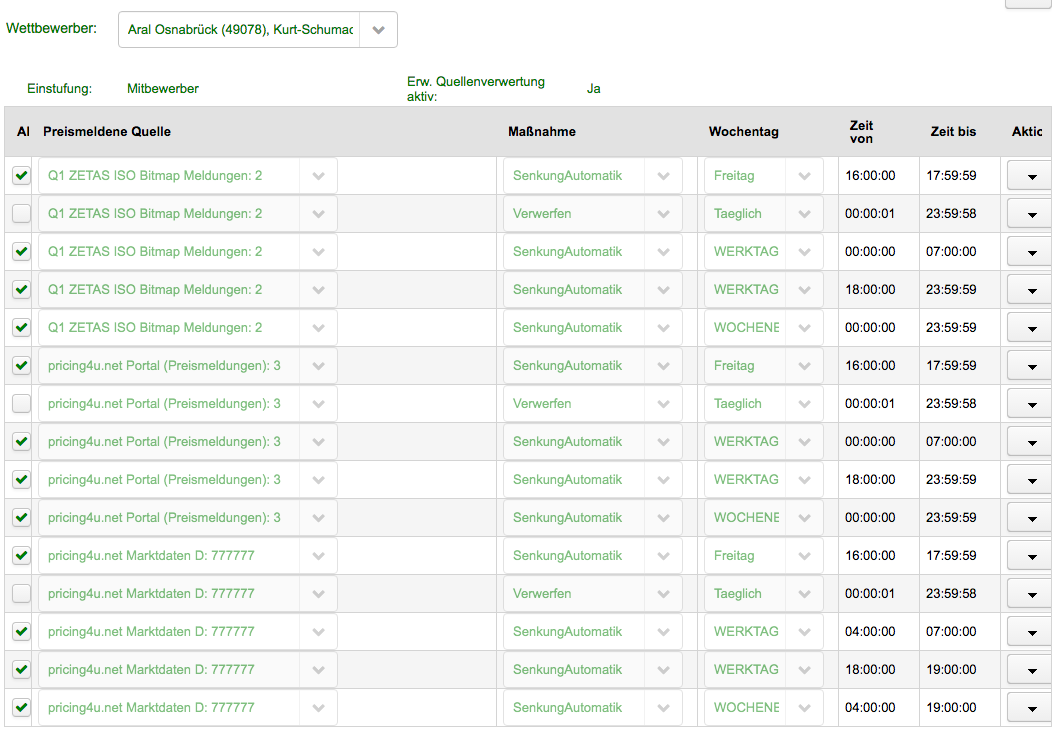
\includegraphics[width=0.8\textwidth]{Bilder/automatik.png}\\
	\captionof{figure}[PT-A]{Princing Tool Automatik Einstellung}
	\label{fig:PT-A}
\end{center}                                                                          
Das Tool bietet neben einer \textit{default} Variante die beiden weitere Möglichkeiten \textit{SenkungAutomatik} und \textit{Verwerfen} an, welche auf unterschiedliche Weise auf Regelverletzungen reagieren. Bei der default Variante wird bei einer Regelverletzung nach der festgelegten Reaktionszeit eine eigene Preisänderung vorgeschlagen, die den niedrigsten tolerierten Preisabstand wieder herstellt. Der Vorschlag kann dann vom Nutzer nach eigenem Ermessen durchgeführt, abgeändert oder gänzlich verworfen werden. Bei der automatischen Senkung wird statt dem Vorschlag die entsprechende eigene Preisänderung nach der festgelegten Reaktionszeit automatischen durchgeführt. Die letzte Möglichkeit verwirft die entsprechende Änderung ohne den Nutzer darüber zu informieren.  Wie auch schon bei den Regeln kann hier für jeden Wochentag für jedes beliebige Zeitintervall eingestellt werden, wie auf einen Verstoß reagiert werden soll.

\pagebreak


% ----------------------------------------------------------------------------------------------------------
% Anforderungsanalyse
% ----------------------------------------------------------------------------------------------------------
\lhead{Anforderungsanalyse}
\titlespacing{\section}{0pt}{12pt plus 4pt minus 2pt}{-6pt plus 2pt minus 2pt}
\section{Anforderungsanalyse}
Thema dieses Abschnittes ist es, das Ziel der Arbeit genau zu spezifizieren und zu modularisieren. Das heißt das Ziel soll bereits in logische Untereinheiten unterteilt werden. Dafür müssen bereits absehbare Probleme erkannt ud notwendige Zwischenergebnisse definiert werden.

\titlespacing{\subsection}{0pt}{12pt plus 4pt minus 2pt}{-6pt plus 2pt minus 2pt}
\subsection{Zielsetzung}
Ziel ist es in den Pricingdaten Verhaltensmuster zu erkennen. Es soll in dieser Arbeit ausschließlich um das Erkennen von reaktivem Verhalten gehen. Das heißt, es geht darum zu erkennen nach welchen anderen Tankstellen sich eine Tankstelle in welchem Maße richtet. Dabei wird sich stark an dem Konzept des vorgestellten Tools orientiert. Es ist anzunehmen, dass Tankstellen, die nicht speziell dieses Tool verwenden, entweder ein sehr ähnlich gestaltetes Tool betreiben oder aber manuell nach ähnlichen Prinzipien operieren.\\
Das liegt an den Grundlagen des Wettbewerbes. Für eine Tankstelle geht es darum, einen möglichst hohen Umsatz an Kraftstofflitern zu einem möglichst hohen Preis zu erzielen. Die für den Kunden interessanten Faktoren sind hierbei in erster Linie der Preis und die Nähe, wobei sich die Gewichtung dieser Faktoren zwischen verschiedenen Kunden und zu verschiedenen Zeiten unterscheidet. Das generelle Kundenaufkommen ist abhängig vom Verkehrsfluss, unterscheidet sich also täglich wie stündlich und teilweise auch saisonbedingt. Es sollte also im Interesse einer Tankstelle liegen, zu den konkurrierenden Tankstellen einen bestimmten Preisabstand zu waren, den es unter Umständen zeitlich zu variieren gilt. Demnach sind die Parameter nach denen in dieser Arbeit gesucht werden soll die jeweilige Konkurrenten einer Tankstelle sowie die gewünschten Preisabstände innerhalb bestimmter Zeitintervalle, was ziemlich genau den Einstellungsoptionen des Tools entspricht.\\
Ein weiterer Grund sich an den Regeln der Tools zu orientieren besteht darin, dass an tatsächlich in den Tools verwendeten Regeln die Performance des verwendeten Ansatzes überprüft werden kann. Das bedeutet nicht, dass das Ziel dieses ersten Ansatzes bereits sein soll die verfügbaren Regelsätze zu hundert Prozent nachzubilden. Es geht immernoch primär darum, die aus dem tatsächlichen Verhalten ersichtlichen Reaktionsmuster zu erkennen. Das dies ein Unterschied ist wird im weiteren Verlauf deutlich werden. Die Regeln sollen zunächst nur dabei helfen auf ansatzweise valide Ergebnisse zu testen.

\titlespacing{\subsection}{0pt}{12pt plus 4pt minus 2pt}{-6pt plus 2pt minus 2pt}
\subsection{Generelle Voranalyse}
Im Bereich der Mustererkennung gibt es ein paar kritische Faktoren, welche besonders ausschlaggebend sind für das prinzipielle Vorgehen. Zunächst muss die Menge der Daten evaluiert werden. Während bei großen Datenmengen die Geschwindigkeit und der verbrauchte Speicher zu kritischen Faktoren werden, sinkt bei geringen Datenmengen schnell die Aussagekraft. Zudem haben Anzahl, Abgrenzung und Konsistenz der Muster einen großen Einfluss auf die benötigte Datenmenge. Es muss auch geklärt werden welche Daten in welcher Form benötigt werden und wie mit fehlenden und fehlerhaften Werten umgegangen werden soll. Zuletzt müssen anhand der Beschaffenheit des Problems, der Verfügbarkeit von Trainingsdaten und der Auswertung der genannten Faktoren mögliche Lösungsansätze ermittelt werden.

\titlespacing{\subsubsection}{0pt}{12pt plus 4pt minus 2pt}{-6pt plus 2pt minus 2pt}
\subsubsection{Datenmenge}
Der Datensatz besteht aus knapp 15000 Tankstellen und insgesammt gut 80 Millionen Preismeldungen, erfordert also aufgrund seiner Größe eine Vorstrukturierung. Eine erste Selektion der Daten ist allein durch die Struktur der gesuchten Muster bereits gegeben. Es werden preisliche Korrelationen zwischen jeweils zwei Tankstellen vermutet, was die Menge durchschnittlich auf  circa 5000 Preisänderungen pro Tankstelle reduziert. Hinzu kommt, dass konkurrierende Tankstellen nicht nur eine Regel haben müssen nach der sie aufeinander reagieren. In Anlehnung an die Funktionen des Pricing Tools wäre es möglich, dass verschiedene Regeln nach einiger Zeit wechseln, für bestimmte Tage definiert sind oder sogar nur für bestimmte Uhrzeiten.\\
Einmal angenommen eine Tankstelle würde für ein halbes Jahr eine Regel für eine Stunde für einen bestimmten Wochentag festlegen. Dann würden durchschnittlich lediglich knapp acht Änderungen in den relvanten Zeitraum fallen. Weiterhin seien alle diese Änderungen reaktive Preissenkungen und die Tankstelle hätte vier gleichwertige Konkurrenten. Dann wären es noch zwei Preisänderungen, die dieser Regel entsprechen würden. Abgesehen davon ,dass die Tankstelle auch noch die Möglichkeit hat die eigenen Regeln zu ignorieren, wären das viel zu wenig Daten um eine statistisch signifikante Aussage treffen zu können. Hier is auch noch nicht berücksichtigt, dass auch genau diese zwei Änderungen als Reaktionen auf diesen Konkurrenten erkannt werden müssen.\\
Die hohe Anzahl der durch die Flexibilität in den Zeitintervallen theoretisch möglichen Regeln macht es also notwendig ein paar Einschränkungen zugunsten signifikanterer Ergebnisse vorzunehmen.

\titlespacing{\subsubsection}{0pt}{12pt plus 4pt minus 2pt}{-6pt plus 2pt minus 2pt}
\subsubsection{Strukturierung des Datensatzes}
Die Datenanalyse soll in Python durchgeführt werden. Die Daten müssen also zunächst von der Datenbank importiert werden. Aufgrund der Menge der Daten, sollten nur diejenigen importiert werden, die für die Analyse einer Tanstelle benötigt werden, um den Arbeitsspeicher nicht zu überlasten. Die Daten sollten so in Python abgespeichert werden, dass besonders einfach und schnell auf die benötigten Datensätze zugegriffen werden kann. Dazu muss herausgearbeitet werden, nach welchen Kriterien besonders häufig auf Daten zugegriffen wird. Es muss auch untersucht werden, ob zusätzliche Daten notwendig oder Datenfelder unnötig sind. Auch die jeweiligen Datentypen  der einzelnen Felder müssen eventuell geändert werden.\\
Da die Daten zu einer Preisänderung von den Tankstellen selber angegeben werden, gibt es ein paar strukturelle Unterschiede in den Angaben. Zunächst ist es möglich pro Kraftstoffsorte eine eigene Preisänderung vorzunehmen, oder aber die Änderungen in Gruppen oder alle zusammen in einem Pricing durchzuführen. Dann gibt es Tankstellen, die vor jeder Änderung den Preis zunächst erst einmal auf Null setzen, bevor sie ihn wieder auf den eigentlich gewünschten Stand anheben. Auch senken einige Tankstellen den Preis bei Tagesende auf Null herab. In einigen Fällen werden Preise für die selbe Kraftstoffsorte in kürzester Zeit mehrmals geändert. Alle diese Vorgehensweisen haben potentiell verschiedene Auswirkungen auf eine automatische Analyse. Es muss einerseits überprüft werden, ob Differenzen unnötigt sind und im Vorhinein angeglichen werden können oder aber wichtige Informationen enthalten und deshalb bewahrt und verschiedenartig behandelt werden müssen. Andererseits muss auch untersucht werden inwiefern diese Auswirkungen im späteren Verlauf zu Problemen führen könnten. Letzteres sollte auch im Bezug auf fehlerhafte, fehlende oder wenig sinnvolle Daten geschehen.\\

\titlespacing{\subsubsection}{0pt}{12pt plus 4pt minus 2pt}{-6pt plus 2pt minus 2pt}
\subsubsection{Algoritmen und andere Ansätze}
Generell geht es bei der Aufgabe darum zu entscheiden, ob eine bestimme Tankstelle auf einer andere reagiert. Demnach ist es unter anderem auch ein Klassifizierungsproblem. Die konkreten Regeln selbst können nicht eindeutig kategorisiert und klassifiziert werden, da sie in ihrer Form zu variabel sind. Allerdings resultieren die Regeln in einzelnen Reaktionen der Tankstellen aufeinander. Man könnte versuchen zu klassifizieren ob eine einzelne Preisänderung die Reaktion auf eine bestimme andere Preisänderung ist. Im anschließend resultierenden Set an Reaktionen, könnte dann nach den spezifischen Regeln gesucht werden.\\
Eine Möglichkeit Reaktionen zu klassifizieren wäre es Methoden aus dem Bereich des maschinellen Lernens zu benutzen. Diese Methoden benötigen zum Erstellen eines Models, welches über die einzellnen Daten entscheidet, klassifizierte Trainingsdaten.
Als Trainingsdaten stehen nur wenige exemplarische Regeln eines einzigen Tankstellenunternehmens zur Verfügung. Man könnte mittels dieser Regeln einige Reaktionen aus dem Datensatz extrahieren. Dies wäre jedoch kein repräsentativer Auszug aus dem Datensatz, da einerseits zu wenige Regelsätze zur Verfügung stehen und andererseits nur das Verhalten eines Anbieters enthalten ist. Das Model würde also selbst wenn die Menge der Trainingsdaten ausreichend wäre nur die Charakteristiken im erhalten einer Tankstelle lernen und wäre damit nicht auf die restlichen Daten übertragbar.\\
Als Alternative dazu könnte man die Reaktionen als kausale Verkettungen betrachten und die entsprechenden Zeitreihendaten mittels statistischer Methoden auf Korrelationen untersuchen. Zur Analyse von Kausalität in Zeitreihendaten werden oftmals verschiedene Variationen des Granger Causality Tests verwendet. Bei diesem Test wird generell geprüft ob zwei Zeitreihendaten in kausaler Relation stehen. Zeitreihe A wäre kausal abhängig von Zeitreihe B, wenn die Vorhersage des jeweils nächsten Wertes in Zeitreihe A signifikant verbessert werden würde, wenn man als Parameter neben den vorherigen Werten von A auch die vorherigen Werte aus der Zeitreihe B hinzunimmt. Für einen solchen Test müssten zunächst Zeitreihendaten generiert werden. Da Reaktionen innerhalb von kürzester Zeit erfolgen können müssten geringe Zeitintervalle gewählt werden. Das würde zu Zeitreihen mit fast ausschließlich gleichen Werten führen, weil der Preis oft über mehrere Stunden gleich bleibt. Ein Vorhersagemodel, was immer den gleichen Preis vorhersagt wäre also nicht mehr signifikant zu übertreffen. Man könnte versuchen dieses Problem zu umgehen und die Zeitintervalle in denen keine Änderung stattfindet ausschneiden. Allerdings wollen Tankstellen vermutlich lediglich einen bestimmten Preisabstand waren und reagieren demnach nicht konsistent auf absolute Preise, sondern nur auf den Anteil der eine bestimmte Preisdifferenz aufweist. Zudem könnten unterschiedliche Abstände sich immer wieder ablösen, sodass zunächst die Daten verschiedenartig in unterschiedliche Zeitfenster unterteilt werden müsste.\\
Bei dieser Vielzahl an Faktoren nach denen die Daten vorselektiert werden müssten, machen die meisten generellen Algorithmen wenig Sinn. Eine eigens auf diese Problemstellung zugeschnittene logische Struktur zu entwickeln scheint am zielführensten. Die Regeln sind inhaltlich über einen Preisabstand definiert. Es sind also nicht absolute Preise, sondern die Differenzen zu den Konkurrenten die wirklich entscheidend sind. Es sollte also eine detailliert Analyse über diese Differenzen durchgeführt werden. Auch ist nicht jeder Differenzwert gleich interessant. Besonders wichtig sind im Konkurrentenverhältnis die vergleichsweise hohen Preisabstände. Dabei ist hier nicht der absolute Betrag gemeint. Die Differenz wird aus dem Blickwinkel der reagierenden Tankstelle errechnet, wobei negative Werte bedeuten, dass diese Tankstelle einen niedrigeren Preis aufweist als der jeweilig betrachtete Konkurrent. Hohe Differenzen bedeuten für die reagierenden Tankstellen als einen verhältnismäßig ungünstigen Preisabstand, wenn mit ungünstig hier die Attraktivität für Kunden gemeint ist. Der in der Regel festgelegte Preisabstand bildet also einen maximalen Schwellenwert. Bei Überschreitung, wird der eigene Preis auch angepasst um den maximalen Schwellenwert wieder herzustellen. Die maximal vorkommenden Differenzen sind also, sofern keine Ausreißer, der Schwellenwert der Regel. Dabei ist es genauso wichtig, die Preisänderungen der Konkurrenten auf welche nicht reagiert wurde zu untersuchen, wie auf die tatsächlichen Reaktionen. Auch hier bilden die maximalen Werte den Schwellenwert der Regel. Dabei muss zusätzlich berücksichtigt werden, dass für unterschiedliche Zeitintervalle unterschiedlich hohe Schwellenwerte hinterlegt seien könnten. Eine detaillierte Analyse der Differenzen zweier Tankstellen ist vor dem Hintergund dieser Vorüberlegungen vom Ansatz her am vielversprechensten. 

\titlespacing{\subsection}{0pt}{12pt plus 4pt minus 2pt}{-6pt plus 2pt minus 2pt}
\subsection{Modularisierung}
Aufgrund der großen Datenmenge sollten die Tankstellen einzeln analysiert werden können, anstatt alle in einem Durchlauf abzuarbeiten. Auch wenn es eventuell möglich wäre die Konkurrenten einer Tanstelle einzeln zu analysieren, ist es unter Umständen hilfreich alle potentiellen Konkurrenten gleichzeitig zu untersuchen. Da nur jeweils eine Preisänderung pro eigenem Pricing als Auslöser in Frage kommt, könnten so verschiedene potentielle Auslöser verglichen werden. Aus diesem Grund wird die Analyse einer Tankstelle auch nicht direkt zweiseitig durchgeführt. Damit wäre gemeint, für eine Tankstelle sowohl die Reaktionen auslösenden Tankstellen, als auch die auf diese Tankstelle reagierenden Tankstellen zu ermitteln. In Verbindung mit dem Ansatz alle potentiell auslösenden Tankstellen gleichzeitig zu untersuchen würde eine zweiseitige Betrachtung zu größeren Verkettungen führen, da bei der Analyse der reagierenden Tankstellen auch wieder deren komplettes Set an möglichen Auslösern verglichen werden müsste. Deshalb werden nur die Reaktionen auslösenden Konkurrenten eines Standortes bestimmt. Zudem kann ein Zeitraum angegeben werden, für den die Analyse einer Tanstelle durchgeführt werden soll.\\
Um nicht alle anderen 15000 Tankstellen anhand ihres tatsächlichen Verhaltens überprüfen zu müssen, sollte eine erste Vorauswahl getroffen werden. Alle wirklichen Konkurrenten auszuwählen hat dabei höhere Priorität als die Auswahl gering zu halten. Anschließen müssen für jede eigene Preisänderung die möglichen Auslöser der potentiellen Konkurrenten ermittelt werden. Zudem werden bei jedem potentiellen Konkurrenten die Preisänderungen ermittelt, auf die nicht reagiert wurde, sowie der jeweilige eigene Preisstand zu diesem Zeitpunkt. Für die Summe aller Preispaarungen pro Tankstellenpaar wird dann die Verteilung der Preisdifferenzen gebildet. Von den Maximalwerten abwärts wird dann auf mögliche Regeln überprüft.

% Ausreißer
% Verschieden Pricing vorgehen und Auswirkungen

\pagebreak

% ----------------------------------------------------------------------------------------------------------
% Umsetzung
% ----------------------------------------------------------------------------------------------------------
\lhead{Umsetzung}
\titlespacing{\section}{0pt}{12pt plus 4pt minus 2pt}{-6pt plus 2pt minus 2pt}
\section{Umsetzung}

\titlespacing{\subsection}{0pt}{12pt plus 4pt minus 2pt}{-6pt plus 2pt minus 2pt}
\subsection{Datenaufbereitung}
Mit Hilfe des Python Modules \textit{psycopg2} werden die benötigten Daten aus der Datenbank nach Python importiert. 

\titlespacing{\subsubsection}{0pt}{12pt plus 4pt minus 2pt}{-6pt plus 2pt minus 2pt}
\subsection{Tankstellendaten}
Der komplette Datensatz an Stammdaten zu den einzelnen Tankstellen wird als Instanzen der Klasse \textit{station} in einem \textit{dictionary} abgelegt, sodass jede Tankstelle über ihre \textit{id} abgerufen werden kann. Jedes einzelne Feld wird entweder übernommen oder, falls nicht verfügbar, mit einem Defaultwert gekennzeichnet. Der großteil der benötigten Funktionalitäten wird über diese Klasse \textit{station} bereitgestellt.  

\titlespacing{\subsection}{0pt}{12pt plus 4pt minus 2pt}{-6pt plus 2pt minus 2pt}
\subsubsection{Preisdaten}
Die für die Analyse benötigten Preisdaten einer Tankstelle werden in einer Matrix chronologisch gespeichert. Bis auf die Tanstellen-Id werden alle Felder übernommen. Der Zeitstempel wird in Zahlenwerte für das Datum und die Uhrzeit umgerechnet. Das Datum besteht in dem Abstand zum Datum der ersten Änderung in Tagen und die Uhrzeit in den an dem Tag vergangenen Sekunden. Zu dem Datum werden zusätzlich der Wochentag und der Monat bestimmt. Zu den jeweiligen aktuellen Preisen werden auch die Änderungsbeträge für jede Kraftstoffsorte ermittelt. Jede Form der Preisänderung wird bis auf einen Außnahmefall so erhalten, wie sie ist. Die Struktur ist von Bedeutung, wenn es darum geht inhaltlich zu bestimmen, welche Änderungen potentiell ein Auslöser seien könnten. Die Ausnahme besteht darin, wenn Preise auf Null herabgesenkt werden. Diese Fälle würden extreme Differenzwerte erzeugen, welche in der Ermittelung der Schwellenwerte für die Regeln Fehler erzeugen könnten. Außerdem stellen sie inhaltlich keine wirkliche Preisänderung dar. In diesen Fällen wird für die entsprechende Kraftstoffsorte der bis dahin geltende Preis genommen. Würde durch diese Abwandlung eine Pricing entstehen, das keine Änderung beinhaltet, so wird der komplette Eintrag entfernt.

\titlespacing{\subsection}{0pt}{12pt plus 4pt minus 2pt}{-6pt plus 2pt minus 2pt}
\subsection{Potentielle Konkurrenten ermitteln}
Wie in der Vorüberlegung angedeutet, soll hier zunächst eine grobe Auswahl der überhaupt als Konkurrenten in Frage kommenden anderen Tankstellen getroffen werden. Das Hauptkriterium hierfür soll der Abstand zur untersuchten Tankstelle sein, welcher über die Geokoordinaten bestimmt werden kann. Dafür wird der Einfachheit halber der direkte Abstand ueber die Erdkugel errechnet. Es ist allerdings nicht ausreichend einfach einen maximalen Abstandswert festzulegen und alle im Umkreis liegenden Tankstellen als potentielle Konkurrenten zu betrachten. Die Anzahl der umliegenden Tankstellen schwankt stark mit dem Besiedelungsgrad der unmittelbaren Umgebung und somit auch die maximalen Abstände von tatsächlichen Konkurrenten. So kann es in der Stadt durchaus vorkommen, dass der nächste Konkurent auf der anderen Straßenseite zu finden ist und sich noch 15 oder mehr weitere Tankstellen im Umkreis von wenigen Kilometern befinden, wohingegen es beispielsweise auf der Autobahn vorkommen kann, dass die nächste Tankstelle mehr als zehn Kilometer entfernt liegt.\\
In der aktuellen Version wird deshalb eine Mischung aus einer Variablen Abstandsobergrenze, einer Mindestanzahl und einer maximalen Anzahl an potentiellen Konkurrenten verwendet. Solange im Umkreis der Obergrenze nicht genügend Tankstellen gefunden wurden, wird die Obergrenze von anfänglich fünf Kilometern immer wieder verdoppelt. Sollte die maximale Anzahl überschritten werden, so werden von den am weitesten entfernten die Überzähligen entfernt. Die so ermittelten potentiellen Konkurrenten werden als Liste ihrer \textit{ids} nach dem Abstand geordnet im der gerade analysierten Station abgespeichert. Grund für dieses Vorgehen anstatt lediglich einer hohen Mindestzahl ist das nicht unnötig viele Tankstellen ausgewählt werden sollen. Bei jeder Tankstelle besteht ein relativ hohes Risiko Korrelationen zu finden, die über Kettenreaktionen und Interaktionen mit dritten Tankstellen hervorgerufen werden. Weitere Möglichkeiten werden im Fazit kurz angesprochen.

\titlespacing{\subsection}{0pt}{12pt plus 4pt minus 2pt}{-6pt plus 2pt minus 2pt}
\subsection{Reaktionen erkennen}
Grundsätzlich wird hier durch die Preisänderungen der untersuchten Tankstelle und der potentiellen Konkurrenten durchiteriert und nach den im folgenden beschriebenen Kriterien Reaktion und deren Auslöser extrahiert. Dabei werden Preiserhöhungen, sowie Preissenkungen kurz nach einer Erhöhung, nicht miteingeschlossen. Anstatt Kopien der Änderungen selber werden die Indexe der Paarungen in ihren Matrizen in Listen gespeichert, einerseits um Arbeitsspeicher zu sparen und andererseits um den historischen Kontext schnell herleiten zu können. Dabei wird je eine Liste für die potentiellen Konkurrenten erstellt um schnell und einfach die Statistiken für die Regeln ableiten zu können, sowie eine chronologisch sortiert nach den Reaktionen mit Unterlisten für alle potentiellen Auslöser um diese später Untereinander vergleichen zu können.\\
Es geht an dieser Stelle noch nicht darum ausschließlich die genauen Auslöser der Preissenkungen einer Tankstelle zu finden. Dazu gibt es nicht ausreichend eindeutige Informationen. Es geht vielmehr darum alle potentiellen Auslöser zu sammeln um darüber anschließen mit statistischen Mitteln die wahrscheinlichsten Konkurrenten und die mit ihnen verbundenen Regeln ermitteln zu können. Dabei ist es unumgänglich  Änderungen als Auslöser zu interpretieren, die prinzipiell in Frage kämen, jedoch tatsächlich nicht wirksam wurden, weil die festgelegte Preisschwelle durch sie nicht unterschritten wurde, da diese Schwelle noch nicht bekannt. Diese Fälle sind aber auch nicht besonders kritisch, da die maximalen Differenzen zu einem potentiellen Konkurrenten zuerst untersucht werden.\\
Probleme können entstehen, wenn auf einem engen Zeitraum mehrere Senkungen vollzogen werden und falsche Paarungen von Reaktionen und Auslösern gemacht werden, weil so potentiell systematisch höhere Differenzwerte als die Schwellenwerte entstehen könnten, die dann statistisch signifikant werden könnten. Deswegen wird bei solchen Fällen eine extra Fallunterscheidung durchgeführt. Ausreißer kann es durch bewusste Regelverletzungen oder technische Ausfälle natürlich trotzdem geben. Diese sollten jedoch so sporadisch sein, dass man sie als eben solche Ausreißer erkannen können sollte. Zunächst werden Reaktionen jedoch nach einer zeitlichen und einer semantischen Komponenten ausgewählt.

\titlespacing{\subsubsection}{0pt}{12pt plus 4pt minus 2pt}{-6pt plus 2pt minus 2pt}
\subsubsection{Zeitliche Komponente}
Auslöser und Reaktion sollten zeitlich nahe beieinander liegen. Das heißt es muss ein maximales Zeitfenster vor einer Preisänderung festgelegt werden, in welchem ein Pricing von einem potentiellen Konkurrenten als Auslöser in Frage kommt. In den letzten Monaten gab es häufig sechs bis acht Preisänderungen verteilt über ein Zeitintervall von weniger als 16 Stunden. Bei Reaktionen mit mehr als zwei Stunden Verzögerung wäre es also nicht unwahrscheinlich, dass die auslösende Tankstelle bereits eine erneute Senkung durchgeführt hat, bevor die Reaktion eintritt. Selbst bei einer Stunde würde bereits ingesammt mehr Zeit bei einem eigentlich ungewünschten Preisabstand verbracht werden als bei dem eigentlich angestrebten. Stark verzögerte Reaktionen sollten somit aus ökonomischer Sicht vermieden werden, um beim Kunden den Eindruck zu vermeiden, dass die Tankstelle verhältnismäßig teurer ist.\\
Trotzdem kann bei automatischen Pricing Tools eine Reaktionszeit eingestellt werden. Die in den Testdaten verwendeten Zeiten sind nicht größer als zehn Minuten. Andere Tankstellen könnten aber durchaus auch höhere Reaktionezeiten eingestellt haben. Tankstellen, die keine Pricing Tools benutzen, haben höchstwahrscheinlich generell eine höhere Reaktionszeit. Zeitenfenster unter 20 Minuten zu verwenden, würde also mit ziemlicher Sicherheit einige Reaktionen nicht berücksichtigen. Um dem vorzubeugen wurde ein Zeitfenster von 45 Minuten gewählt. Ein zu großes Zeitfenster würde dazu führen mehr korrelierende, aber nicht kausal verantwortlich, Preisänderungen in den Pool der potentiellen Auslöser aufzunehmen.

\titlespacing{\subsubsection}{0pt}{12pt plus 4pt minus 2pt}{-6pt plus 2pt minus 2pt}
\subsubsection{Semantische Komponente}
Inhaltlich sollte der Höhenbetrag der Änderung in allen geänderten Kraftstoffsorten bei der Reaktion kleiner oder gleich der Änderung des Auslösers sein. Das liegt daran, dass der Preisabstand vor einem Auslöser maximal dem Schwellenwert entspricht. Ein Auslöser kann den Schwellenwert also maximal um die Höhe seiner Änderung unterschreiten. Eine Reaktion die den Schwellenwert wieder herstellt darf also nicht höher Ausfallen als der Auslöser selber. Hier wird auch deutlich warum die verschiedenen Strukturen des Pricings beibehalten werden sollten und nicht etwa ein Datensatz für jede Kraftstoffsorte erstellt wurde. Entspricht nur eine Kraftstoffsorte einer Preisänderung nicht notwendigen Kriterien, so kommt die ganze Änderung als regelkonforme Reaktion nicht mehr in Frage. Bei einzelner Betrachtung der Kraftstoffsorten wäre diese Verschärfung des Ausschlusskriterium nicht möglich gewesen.\\

\titlespacing{\subsubsection}{0pt}{12pt plus 4pt minus 2pt}{-6pt plus 2pt minus 2pt}
\subsubsection{Fallunterscheidung}
Es gibt vier verschiedene Fälle, die durch die verschiedenartigen Strukturen im Pricing Verhalten aber noch verkompliziert werden. Generell soll es möglich sein, dass ein Auslöser mehrere Reaktionen hervorruft und zwar maximal eine pro Kraftstoffsorte. Umgekehrt gilt das Gleiche, also das mehrere Auslöser eine Reaktion hervorrufen. Das liegt daran, dass es denkbar wäre dass sowohl die verantwortlichen Personen als auch automatische System Pricings mit mehreren Kraftstoffsorten in einer Änderung in ihre Einzelteile aufspalten oder auch Einzelne zu einem Ganzen zusammenfügen. Es soll aber ausgeschlossen sein, dass pro Auslöser-Reaktion-Paarung ein Kraftstoff bei einer Partei mehrmals geändert wird. Bei manuellen Änderungen ist es zwar möglich, dass bei einer Anpassung Fehler unterlaufen und deswegen eine weitere hinzugefügt werden muss, doch sollten diese Fälle so vereinzelt sein, dass es das Ergebnis nicht beeinflussen sollte. Auslöser-Reaktion-Paarungen können also maximal drei Änderungen pro Seite enthalten. Zudem können in einem Zeitfenster verschieden viele unabhängige Preisänderungen auf beiden Seiten stattfinden. Deshalb werden pro Seite die beiden Kategorien eine Preisänderung oder mehrere unterschieden, sodass sich aus den verschiedenen Kombinationen insgesammt vier verschiedene Fälle unterscheiden lassen. 

\begin{enumerate}
\item [\textbf{ein Auslöser - eine Reaktion}]
Die am häufigsten vorkommende Variante. Hier muss nur die semantische Komponente überprüft werden. 
\item [\textbf{ein Auslöser - mehrere Reaktionen}]
In diesem Fall befindet sich nur eine einzelne potentiell auslösende Preisänderung aber mehrere Preisänderungen der untersuchten Tankstelle in einem Zeitintervall. Die letztlich gewählte Reaktion sollte auf jeden Fall das semantische Kriterium erfüllen. Bei den späteren Reaktionen muss für die Überprüfung dieses Kriteriums die Summe aller vorherigen Änderungen in diesem Zeitintervall auf die jeweilige Reaktion selber draufaddiert werden. Denn falls eine der späteren Änderungen die tatsächliche Reaktion war, dann war sie trotz allen vorherigen, ohnehin schon durchgeführten, Änderungen anscheinend immernoch erforderlich. Es wird hierbei davon ausgegangen, dass auch die automatischen Tools nach dem Abwarten der Reaktionszeit vor der Durchführung der eigenen Änderung noch einmal den zu ändernden Betrag überprüfen. Würden sie dies nicht tuen, könnte das dazu führen, dass eine Tankstelle systematisch einen geringeren Preis als nötig fährt und somit Gewinne einbüßt. Deshalb werden die potentiellen Reaktionen, angefangen bei der Ersten, aufaddiert, bis das semantische Kriterium nicht mehr erfüllt wird. Die letzte Änderung die das Kriterium noch erfüllt wird als tatsächliche Reaktion eingestuft. Wenn diese Änderung alleine nicht alle Kraftstoffsorten die beim Auslöser geändert wurden abdeckt, können vorherige noch hinzugenommen werden, sofern sie nicht zu einer doppelten Änderungen einer Sorte führen würden.\\
Es ist nicht möglich die früheren Reaktionen inhaltlich komplett auszuschließen. Die Früheren zu wählen würde aber einen höheren Schwellenwert unterstützen. Die späteren Reaktionen sind, weil sie vorheringen in dieser Hinsicht implizieren summiert größerer Anpassungen, stellen also letztlich wieder eine niedrigere Differenz her. Es ist also sicherer die Reaktionen zu nehmen die bei gleichzeitigem Erfüllen des semantischen Kriteriums am spätesten sind, um nicht das Risiko einzugehen unsichere größere Schwellenwerte zu begünstigen. Außerdem ist dieses Szenario extrem unwahrscheinlich. Der Auslöser, der mehrere Reaktionen erklären kann, also an sich schon hohe absolute Senkungen umfasst, mindestens zwei Cent, löst nur die frühere Reaktion aus. Es muss also in kürzester Zeit noch einen weiteren Preisverfall geben, der den bisherigen noch einmal unterschreitet um die weiteren Anpassungen zu rechfertigen. Der Preis würde also in kürzester Zeit um mindestens 3 Cent verfallen. Es sollte im Interesse keiner Tankstelle sein hohe Preisverfälle zu erzeugen.\\
PROBLEM: Angenommen es kommt zunächst eine Reaktion die gegen das semantische Kriterium verstößt, weil sie einen Preis ändert der vom Auslöser nicht verändert wurde, so würde gar keine Reaktion gewählt obwohl spätere durchaus die wahren Reaktionen sein könnten.

\item [\textbf{mehrere Auslöser - eine Reaktion}]
Der umgekehrte Fall, bei welchem mehrere Änderungen eines Konkurrenten einer einzelnen Reaktion vorausgehen, lässt eine eindeutigere Entscheidung zu. In diesem Fall ist die letzte semantisch plausible Änderung des Konkurrenten der potentielle Auslöser. Angenommen eine vorherige Änderung hätte die Reaktion ausgelöst, dann hätten alle noch folgenden Änderungen wiederum Reaktionen auslösen müssen. Es erfolge jedoch offenbar nur eine. Zudem ist diese Lösung wieder die sichere Variante. Bei den späteren Änderungen sind schon mehr Senkungen erfolgt, der Konkurrent hat also einen niedrigeren Preis. Die Reaktion stellt hier also einen verhältnismäßig niedrigen Schwellenwert wieder her. Sollte also der Fall eintreten, dass doch eine der früheren Änderungen der Auslöser war und es wurde manuell eine weitere Senkung verhindert, so ist dies zum Einen ein von der Tankstelle gewollter Ausreißer und sollte auch so in den Statistiken auftauchen und zum Anderen auch ein Ausreißer nach unten und somit nicht besonders ausschlaggebend, was die Wahl der Schwellenwerte betrifft.\\
Auch hier muss bei der Auswahl wieder berücksichtigt werden, dass eventuell nur mehrere Änderungen zusammen den Auslöser bilden. Die Auslöser werden deshalb von hinten durchiteriert. Handelt es sich bei dem aktuellen Auslöser um eine Änderung, bei der es keinerlei Überschneidung bei den geänderten Kraftstoffsorten mit der Reaktion gibt, so kann diese Änderung übergangen werden. Das liegt daran, dass diese Änderung auch nicht eine erneute Änderung hätte auslösen müssen. Dies ist jedoch der Fall, sobald es eine solche Überschneidung gibt. Wenn die Änderung mit dieser Überschneidung das semantische Kriterium noch nicht erfüllt können frühere hinzugenommen werden. Wieder dürfen dabei keine doppelten Änderungen einer Kraftstoffsort entstehen.  

\item [\textbf{mehrere Auslöser - mehrere Reaktion}]
Die letzte Variante ist in gewisser Weise eine Kombination der vorherigen Fälle, was sich auch in der logischen Begründung wiederspiegelt. Zunächst wird für die Kombination aller Auslöser untersucht, wieviele Reaktionen dadurch erklärt werden können. Dazu werden die Auslöser zu einem einzelnen künstlichen Auslöser zusammengefasst und dann die Reaktionen der Reihe nach addiert, śolange das semantische Kriterium erfüllt bleibt. Sofern am Ende Reaktionen überbleiben, werden diese mit der selben Begründung, wie im 2. Fall außer acht gelassen. Können alle Reaktionen erklärt werden, ist dies nicht notwendig.\\

Die übrigen Reaktionen werden dann einzeln in rückwärtiger Reihenfolge untersucht und gefunden Paarungen werden für die weitere Untersuchung gelöscht, damit sie nicht doppelt vorkommen. Für diese, durch das Löschen ist sie die jeweils letzte der zu betrachtenden Reaktionen, werden alle davorliegenden Auslöser gesammelt und der 3. Fall wird angewendet. Das Entscheidungskriterium zugunsten des letzten möglichen Auslösers scheint hier außer Kraft gesetzt, denn spätestens ab der zweiten Iteration hatte es ja noch weitere spätere Reaktionen gegeben. Allerdings wurde für diese durch die rückwärtige Analyse bereits ein Auslöser gefunden, oder bewiesen dass es keinen gibt, wodurch dieses Kriterium doch weiterhin gültig ist.\\

Wurden ein oder mehrere Auslöser für die aktuelle Reaktion gefunden muss nur noch überprüft werden, ob weitere Reaktionen zwischen dem letzten der Auslöser und dieser aktuell letzten Reaktion liegen, die zusätzlich durch die aktuell gewählten Auslöser erklärt werden können. Es muss nicht noch einmal die Summe wie im 2. Fall gebildet werden, da diese Notwendigkeit durch die zu allererst gebildete Summe behoben wurde.\\

Dabei kann es rein theoretisch wieder vorkommen, dass Auslöser, die zu einer spätere Reaktion passen, mit diesen gepaart und entfernt werden, obwohl sie eigentlich die Auslöser einer anderen früheren Reaktion sind. Für diese HAndhabung srechen wieder die selben Gründe wie im 2. Fall. Es ist aus ökonomischer Sicht höchst unwahrscheinlich und zudem sicherer eine spätere Reaktion als tatsächliche Reaktion in Betracht zu ziehen, weil dabei weniger kritische Fehler begangen werden.\\
Wurde kein Auslöser gefunden wird nur die gerade aktuell letzt Reaktion gelöscht.
\end{enumerate}

\titlespacing{\subsection}{0pt}{12pt plus 4pt minus 2pt}{-6pt plus 2pt minus 2pt}
\subsection{Regeln spezifizieren}
Aus den gesammelten potentiellen Reaktionen sollen nun die in den Tools hinterlegten Regeln oder aber auch lediglich konsistente Konkurrenzmuster abgeleitet werden. Dazu sollen maximal zugelassene Preisabstände sowie die dazugehörigen Zeitintervalle erkannt werden. Letztlich muss dann über die errechneten Statistiken ermittelt werden, welche Tankstellen wirklich Konkurrenten sind. 

\titlespacing{\subsubsection}{0pt}{12pt plus 4pt minus 2pt}{-6pt plus 2pt minus 2pt}
\subsubsection{Maximaler Preisabstand}
Die Verteilung der Preisdifferenz zweier Tanstellen ist das Hauptkriterium auf welches sich die Klassifikation von Konkurrenz stützen wird. Wurde eine Regel und damit ein Schwellenwert für einen Konkurrenten hinterlegt, so sollte die Differenz nie lange über diesen Wert steigen. Es gibt Zeit Möglichkeiten, wie eine Tankstelle auf die Änderung eines Konkurrenten entsprechend einer Regel reagieren kann. Entweder gar nicht, weil der Schwellenwert nicht überschritten wurde. Oder aber mit einem eigenen Preissenkung weil eben dies der Fall war. Deshalb werden zwei verschiedene Differenzwerte unterschieden. Zum einen der Preisunterschied nach einer Änderung auf die nicht reagiert werden muss. Der Maximalwert beschreibt somit den maximalen Abstand auf den nicht reagiert werden musste, was glechzeitig dem Schwellenwert entspricht. Zum Anderen der Preisunterschied nach einer potentiellen Reaktion. Für den Fall, dass es eine tatsächliche Reaktion und nicht nur eine Korrelation ist, dann sollte nach der reagierenden Preisänderung der Schwellenwert wieder hergestellt worden sein. Bei beiden diesen Differenzen bestimmen die maximalen Werte den potentiellen Schwellenwert einer Regel. Dadurch dass auch Preisänderungen ohne Reaktion in die Daten einfließen und nur Konkurrenten getestet werden, die mindestens ein zehntel der Preisänderungen der untersuchten Tankstelle aufweisen, ist garantiert, dass genügend Daten für eine Analyse vorliegen.\\
Bei der Analyse dieser Werte werden die einzelnen Kraftstoffsorten zum ersten mal komplett getrennt betrachtet. Werden bei einer Reaktion nicht alle Kraftstoffe angepasst so sollten die Gleichgebliebenen eben nicht in die Kategorie Reation, sondern in die der nicht notwendigen Reaktion fallen. Für jeden potentiellen Konkurrenten werden deshalb je zwei Histogramme über die Preisunterschiede pro Kraftstoffsorte erstellt. Das Erste mit Hilfe der Liste aller potentiellen Reaktionen auf einen Konkurrenten. Und das Andere mit allen Preisänderungen eines Konkurrenten die nicht in dieser Liste auftauchen und keine Erhöhungen sind. Jede dafür in Frage kommende Änderung wird noch einmal dahingehend überprüft, ob tatsächlich kein Pricing der untersuchten Tankstelle im anschließenden Zeitfenster zu finden ist. Durch das semantische Kriterium sind schließlich zeitlich korrelierende Anpassungen ausgeschlossen worden, weil sie keine Reaktionen darstellen, wo der Auslöser jedoch auch nicht notwendigerweise einen Preisabstand hergestellt hat, auf den nicht reagiert hätten werden müssen. Es könnte durchaus sein, dass eine Reaktion erforderlich gewesen wäre, hätte nicht sowieso ein anderer Konkurrent eine stärkere Reaktion bewirkt. Zudem müssen für die wirklich ignorierten Änderungen des Konkurrenten noch die gerade geltenden Preise der untersuchten Tankstelle ermittelt werden.\\
Die beiden Histogramme müssen dann für die Bestimmung des Maximalwertes zunächst zusammengerechnet werden. Der dabei entstehende Maximalwerk kann jedoch nicht sofort zum Schwellenwert gemacht werden. Es muss berücksichtigt werden, dass es durchaus noch seien kann, dass Tankstellen die Preise ohne Hilfe eines Tools anpassen, oder zumindest die Anpassung selber noch manuell durchführen. Es kann also vorkommen, dass obwohl eine Regel besteht ab und zu dagegen verstoßen wird. Die Maximalwerte müssen also zunächst auf Ausreißer überprüft werden. Beziehungsweise, es muss überprüft werden, ob die Häufigkeit, mit der ein entsprechender Wert Auftritt regelmäßig genug ist um die Vermutung von konkurierendem Verhalten zu stützen. Diesbezüglich kann es durchaus vorkommen, dass zu einer Tankstelle eine Regel hinterlegt wurde, welcher aber nur sehr selten eine Reaktion erfordert. Es kann zum Beispiel sein, dass der entsprechende Konkurrent selber in erster Linie auf die gerade untersuchte Tankstelle reagiert. Extremfälle dieser Art können nicht berücksichtigt werden, da das tatsächlicher Verhalten diese Regeln nicht rechtfertigt und es somit eher angeraten wäre die Existenz der Regeln zu hinterfragen.\\
Zusätzlich gilt es noch zu berücksichtigen, dass sollte ein Wert zurückgewiesen werden, alle Differenzwerte die diesen Wert gestützt hätten zu Regelverstößen werden würden. Es gibt hierzu allerdings Tankstellenübergreifenden keine Erfahrungswerte, wie oft gegen Regeln verstoßen wird. Es ist durchaus möglich, dass sich dieser Faktor zwischen verschiedenen Unternehmen stark unterscheidet. Grundsätzlich sollte aber davon ausgegangen werden können, dass sich größententeils an Regeln gehalten wird, da diese Regeln einer ökonpmischen Optimierung entstammen und Verstoße generell eine Gefahr bergen Kunden zu verlieren.\\
Zuletzt soll es ja auch möglich für eine Tankstelle sein Regeln auf bestimmte Zeit zu begrenzen, wodurch die Anzahl der diesbezüglichen Reaktionen auch deutlich geringer ausfallen kann. Diese drei Faktoren sprechen dafür schon bei einer recht geringen Anzahl eine Regelmäßigkeit zu vermuten. Als Grenzwertfunktion wurde dafür diese Funktion gewählt:
\begin{center}
$ \frac{2}{\pi}*\arctan(2*\frac{x^2}{y})$ mit x=Häufigkeit, y=Grundgesammtheit\\
\end{center}

Der Grenzwert sollte relativ zu der Menge der in diesem Zeitinterval liegenden Preisänderungen gewählt werden. Um die Häufigkeit des Wertes stärker zu gewichten, wird diese quadriert, damit bei moderat hohen Häufigkeiten eine unverhältnismäßig höhere absolute Anzahl an Preisänderugen nötig wäre um diesen Wert zurückzuweisen. Angenommen es würde einfach eine Prozenthürde von 10\% gewählt so würde bei einer passenden Änderung aus zehn bereits ein Regel vermutet wohingegen 9 aus 100 zurückgewiesen werden würden. Mit dem Arkustangens und den zusätzlichen Faktoren soll der errechnete Wert in einen Konfidenzwert sein also eine Wahrscheinlichkeit zwischen 0 und 1 umgerechnet werden. Während die geringen Werte kaum verändert werden, muss bei den hohen Werten der quadratische Faktor wieder ausgeglichen werden. Die errechneten Konfidenzwerte lassen so trotzdem einen relativ guten Vergleich zwischen verschiedenen Regeln zu. Bei einem Maximalwert wird ab einer Häufigkeit, die einem Konfidenzwert größer als 0.5 entspricht, eine Regelmäßigkeit vermutet. Da es möglich ist, dass Tankstellen für einen Konkurrenten mehrere Regeln mit unterschiedlichen Schwellenwerten zu unterschiedlichen Zeiten erstellen, kann es durchaus vorkommen, dass auch niedrigere Werte noch Regeln darstellen. Deshalb wird bei potentiellen Regeln zunächst überprüft in welchem Zeitfenster sie gültig sind. Solange noch Zeitslots übrig sind in denen noch keine Regel befolgt wird, werden die nächst niedrigeren  Werte untersucht. 

\titlespacing{\subsubsection}{0pt}{12pt plus 4pt minus 2pt}{-6pt plus 2pt minus 2pt}
\subsubsection{Zeitinterval}
Für jeden möglichen Maximalwert müssen nun die Zeitintervalle ermittelt werden, in denen dieser Wert auftritt und somit das Zeitfenster der Regel definieren. Es war zunächst ein Ansatz gedacht gewesen der die Regeln von den Zeitintervallen ausgehend erstellt, statt zunächst ganzheitliche Maximalwerte zu errechnen. Die Daten sollten rekursiv in immer kleinere Zeitintervall aufgespalten und anschließend für jedes Intervall aus den darinliegenden Daten die Maximalwerte errechnet werden. Anschließend sollten die Slots mit gleichen Werten zusammengefügt werden. Dies hat dazu geführt, dass bereits beim Versuch die Daten nach einzelnen Wochentagen und Stunden zu spalten zu wenig Daten für die einzelnen Intervalle zur Verfügung standen um halbwegs sichere Aussagen zu treffen. Auch sind nicht so hochfrequente Konkurrenzmuster gänzlich unerkannt geblieben. In den zu Testzwecken zur Verfügung stehenden Regeln gibt es allerdings auch nur einen Einzelfall an welchem überhaupt eine zeitliche Unterscheidung von Schwellenwerten getroffen wurde. Es gilt zwar wieder, dass diese Testwerte nicht umbedingt repräsentativ für den ganzen Kraftstoffmarkt sind, trotzdem wurde aufgrund dieser Beispiele und zugunsten Aussagekräftigerer Ergebnisse dieser Ansatz verworfen.\\
Stattdessen wird zunächst ein übergreifend gültiger Schwellenwert vermutet. Deswegen werden die Differenzhistogramme über den gesammten Zeitraum gebilten. Anschließend wird ermittelt in welchen Zeitintervallen dieser Maximalwert auftritt. Hierbei wird nur einzeln entweder nach ganzen Tagen, oder nach Stunden unterschieden. Es könnte zwar sein, dass detailliertere Regeln existieren. Aber es ist relativ unwahrscheinlich, dass so eine feine Unterscheidung allzu häufig getroffen wird. Schließlich sollte es für jede weitere Aufsplittung eine ökonomische Rechfertigung geben. Es sind zwar bei genaueren Analysen durchaus unterschiede im Kundenaufkommen an verschiedenen Tages- und Uhrzeiten zu vermuten, allerdings müsste man für eine gänzlich danach ausgelegte Preisstruktur auch annehmen, dass Kunden die Preise so detailliert verfolgen, dass sie ebenfalls die Tankstellen nach diesen Strukturen unterscheiden statt einfach nur die im allgemeinen günstigere oder nächstbeste zu nehmen. Da angenommen werden kann, dass dies nicht der Fall ist und sich eine detaillierter Analyse der Daten sowieso sehr schwierig gestaltet, wird lediglich nach Unterschiede zwischen einzelnen Tagen oder Uhrzeiten, jedoch nicht kombiniert nach beiden untersucht.\\
\paragraph{Potentielle Zeitintervalle ermitteln}
Dafür müssen zunächst alle möglichen Zeitslots für Tage und Stunden ermittelt werden. Dies sind die Zeiten zu denen jeweils die untersuchte Tankstelle und der Konkurrent beide geöffnet haben. Wie eben angesprochen werden nur die Tage und Tageübergreifend eine Stundenanzahl ermittelt. Einzelne unterschiede zum Beispiel am Wochenende werden außer acht gelassen. Die Öffnungszeiten der Tankstellen stehen in dem Datensatz von Tankerkönig nicht zur Verfügung. Allerdings reicht es auch zu ermitteln in welchen Zeitslots beide Tankstellen Preisänderungen durchführen, da diese ohnehin auch nur die Zeitslots sind bei denen Daten zur Verfügung stehen. Es ist außerdem besonders wichtig, dass jeder Zeitslot auch Daten hat an denen er untersucht werden kann, da so lange weitere Schwellenwerte überprüft werden, bis alle Slots belegt sind. Auch hier müssen deswegen wieder Ausreißer berücksichtigt werden. Bei beiden Kategorien Tagen und Stunden werden die \textit{Öffnungszeit} für die an der Analyse betrachteten Tankstellen getrennt ermittelt und anschließend die der untersuchten Tankstelle mit dem jeweiligen Konkurrenten kombiniert (Verundung).\\
Zur Bestimmung der geöffneten Tage wird der Mittelwert an Änderungen der Tage berechnet an denen Änderungen stattfinden. Anschließend wird für jeden einzelnen Tag getestet, ob ein zehntel dieses Mittelwertes überschritten wird um den Tag in die Analyse mit einzuschließen. Das ist notwendig um einerseits Ausreißer auszuschließen und andererseits zusätzlich gewähren zu können, dass die Analyse des jeweilige Maximalwertes für jeden Tag genügend zugrunde liegende Daten aufweist. Die Bestimmung der Stunden läuft bis dahin äquivalent ab. Allerdings müssen hier neben den positiven Ausreißer, also Preisänderungen zu Zeiten in denen die Tankstelle eigentlich nicht geöffnet ist, aber aus irgendwelchen Gründen trotzdem Preise geändert werden auch negativ Ausreißer, also Zeiten in denen die Tankstelle geöffnet hat aber nur sehr wenige oder gar keine Preissenkungen vornimmt, berücksichtigt werden. Auch hier werden die Erhöhungen rausgenommen, da diese oftmals zu Randzeitpunkten wie zu Begin oder am Ende einer Öffnungsperiode stattfinden und dabei öfters aus der tatsächlichen Öffnungszeit rausfallen. Für jede Stunde werden bei der Entscheidung zusätzlich jeweils die drei vorherigen und folgenden Stunden berücksichtigt. Für das vorliegende und nachliegende Intervall werden jeweils die Stunden gezählt bei denen der Grenzwert von einem zehntel vom Mittelwert überschritten wurde. Wird bei der betreffenden Stunde selber dieser Wert überschritten, so wird das Maximum dieser beiden Randintervalle gewählt und für die Entscheidung überprüft, ob mindestens zwei der drei Stunden ebenfalls diesen Wert überschreiten. Wird der Wert für die Stunde selber nicht erreicht, so wird das Minimum der Randintervall dem gleich Test unterzogen. Dieses Verfahren hat den Hintergrund dass es bei den Testtankstellen, hier kann repräsentativ getestet werden, da die Öffnungszeiten generell öffentlich zugänglich sind, innerhalb der Öffnungszeiten Intervalle von maximal zwei Stunden auftreten können zu denen es kaum oder selten auch mal keine Änderungen gibt. Dieses Verfahren ermöglicht es diese Stunden trotzdem in die Analyse mit einzuschließen und gleichzeitig die Ränder nicht zu vergrößern. Zwar gibt es für diese so zusätzlichen Stunden keine Daten, was aber nicht problematisch ist, weil diese Fälle im weiteren Verlauf berücksichtigt werden.\\
\paragraph{Konkrete Zeitintervalle für Regeln definieren}
Wenn die möglichen Zeitslots feststehen, muss für die Schwellenwerte bezüglich eines Konkurrenten ein Gültigkeitsbereich definiert werden. Diese Slots ergeben sich durch die Verteilung derjenigen Reaktionen und ignorierten Preisänderungen, die exakt diesen gerade untersuchten Maximalwert generiert haben. Deshalb wird noch einmal ein Tages- sowie Stundenhistogramm für genau diese Änderungen erstellt, die in diese Kategorie fallen. Es kann sein, dass dieser Schwellenwert so in nicht in jedem Slot vorkommt. Diejenigen Slots bei den nicht sicher genug Reaktionen oder ignoriereten Preisänderungen mit Differenzen in dieser Höhe festgestellt werden, sind Kandidaten für einer weitere schwächere Regel.\\
Damit ein Zeitslot den aktuellen Schwellenwert zugewiesen bekommt müssen ähnliche Probleme, wie auch schon bei der Analyse der generell verfügbaren Slots bedacht werden. Bei der Festlegung der Tage sind die Werte noch dicht genug, dass vom Ablauf her das selbe Verfahren durchgeführt wird mit dem Unterschied, dass dieses mal nicht alle Preisänderungen in Frage kommen sondern nur die dem aktuellen Schwellenwert zugehörigen. Wegen dieser Einschränkung der Datenmenge muss die Analyse bei den Uhrzeiten noch einmal abgewandelt werden. Hier findet eine zu große Teilung der Daten statt dafür dass das Pricingverhalten auch bei normalem regelkonformem Verhalten hier schon größeren Schwankungen unterlegen ist. Der Grenzwert ab dem ein Slot belegt wird ist hier abhängig von der Relation der in diesem Slot liegenden Änderungen der gerade getesteten Höhe zu der Gesammtheit der in diesem Slot liegenden Preisänderungen. Der Anteil sollte 10 Prozent nicht unterschreiten. Auch hier müssen wieder die Schwankungen berücksichtigt werden. Um nicht starkt fluktuierende Regeln zu generieren, das heißt im Extremfall welche die jeweils immer nur für einzelne Stunden gültig sind, wird die Mindestgültigkeitsdauer einer Regel auf 3 Stunden gesetzt. Daraus ergibt sich, dass sowohl einzelne Slots sowohl zusätzlich aufgenommen, als auch trotz hoher Werte zurückgewiesen werden können. Umgesetzt wird dies dadurch dass ein 5 Slots großer Kernel über die Liste der Uhrzeiten laufen gelassen wird, der die Belegung des einzelnen Slots im Zentrum auf den im Kernel häufiger vorkommenden Wert setzt. Nach diesem Schritt sind für jeden Konkurrenten die möglichen Regeln eindeutig definiert.

\titlespacing{\subsubsection}{0pt}{12pt plus 4pt minus 2pt}{-6pt plus 2pt minus 2pt}
\subsubsection{Klassifikation Konkurrenz}
Da aber auch die Abstände bei ignorierten Änderungen eines Konkurrenten verwendet wurden, bedeutet eine Regel noch nicht die Existenz einer Konkurrenz

% \titlespacing{\subsection}{0pt}{12pt plus 4pt minus 2pt}{-6pt plus 2pt minus 2pt}
% \subsection{Automatisierungsgrad bestimmen}

% Wenn man nach dem oben beschriebenen Tool geht, gibt es drei Stufen der Automatisierung. Tankstellen können keines dieser Tools verwenden und auf andere Mittel zurückgreifen. Sie können sich vom Tool Preisänderungen Vorschlagen lassen, diese jedoch manuell nach eigenem ermessen durchführen. Oder sie können das Pricing vollautomatisch durch diese Tools betreiben lassen. Die letzten beiden Methoden können natürlich wieder zeitlich variabel abgewechselt werden. Um diese drei Varianten unterscheiden zu können, müssen die unterschiedlichen Reaktionen aufs Pricing Verhalten analysiert werden. Die höchste Stufe der Automatisierung zeichnet sich dadurch aus, dass die in diesem Zeitraum liegenden Regeln keine Ausnahmen haben und die Varianz der Reaktionszeit äußerst gering ist, da hier automatisch und regelbasiert agiert wird. Bei der nächstniedrigeren Stufe, dem Folgen von Vorschlägen, sollten nur geringfügig Abweichungen zum automatischen Betrieb auftauchen, und zwar in der Form, dass Regeln ab und zu verletzt werden und die Varianz der Reaktionszeit merklich ansteigt. Beim arbeiten ohne diese Tools, kann zwar nicht sicher gesagt werden, nach welchen Kriterien hier gearbeitet wird, es sollte jedoch anzunehmen sein, dass das Verhalten weniger Regelkonform ist und mit höheren Reaktionszeiten einhergeht.


% \titlespacing{\subsubsection}{0pt}{12pt plus 4pt minus 2pt}{-6pt plus 2pt minus 2pt}
% \subsubsection{Formen der Automatisierung}

% \titlespacing{\subsubsection}{0pt}{12pt plus 4pt minus 2pt}{-6pt plus 2pt minus 2pt}
% \subsubsection{Regelverletzung und Reaktionszeiten}

\pagebreak

% ----------------------------------------------------------------------------------------------------------
% Ergebnisse
% ----------------------------------------------------------------------------------------------------------
\lhead{Ergebnisse}
\titlespacing{\section}{0pt}{12pt plus 4pt minus 2pt}{-6pt plus 2pt minus 2pt}
\section{Ergebnisse}

\titlespacing{\subsection}{0pt}{12pt plus 4pt minus 2pt}{-6pt plus 2pt minus 2pt}
\subsection{Beschreibung}

\titlespacing{\subsection}{0pt}{12pt plus 4pt minus 2pt}{-6pt plus 2pt minus 2pt}
\subsection{Diskussion}

\titlespacing{\subsubsection}{0pt}{12pt plus 4pt minus 2pt}{-6pt plus 2pt minus 2pt}
\subsubsection{Statistiken}

\titlespacing{\subsubsection}{0pt}{12pt plus 4pt minus 2pt}{-6pt plus 2pt minus 2pt}
\subsubsection{Problemanalyse}

\titlespacing{\subsection}{0pt}{12pt plus 4pt minus 2pt}{-6pt plus 2pt minus 2pt}
\subsection{Zusammenfassung}


\pagebreak

% ----------------------------------------------------------------------------------------------------------
% Fazit
% ----------------------------------------------------------------------------------------------------------
\lhead{Fazit}
\titlespacing{\section}{0pt}{12pt plus 4pt minus 2pt}{-6pt plus 2pt minus 2pt}
\section{Fazit}

\titlespacing{\subsection}{0pt}{12pt plus 4pt minus 2pt}{-6pt plus 2pt minus 2pt}
\subsection{Weitere Möglichkeiten}

\titlespacing{\subsubsection}{0pt}{12pt plus 4pt minus 2pt}{-6pt plus 2pt minus 2pt}
\subsubsection{Gegenrichtung prüfen}

\titlespacing{\subsubsection}{0pt}{12pt plus 4pt minus 2pt}{-6pt plus 2pt minus 2pt}
\subsubsection{Reaktionen an Regeln trimmen}

\titlespacing{\subsubsection}{0pt}{12pt plus 4pt minus 2pt}{-6pt plus 2pt minus 2pt}
\subsubsection{Auslöser untereinander vergleichen}

\titlespacing{\subsubsection}{0pt}{12pt plus 4pt minus 2pt}{-6pt plus 2pt minus 2pt}
\subsubsection{Constraint Satisfaction}


% \pagebreak

% % ----------------------------------------------------------------------------------------------------------
% % Verzeichnisse
% % ----------------------------------------------------------------------------------------------------------
% % TODO Typ vor Nummer
% \renewcommand{\cfttabpresnum}{Tab. }
% \renewcommand{\cftfigpresnum}{Abb. }
% \settowidth{\cfttabnumwidth}{Abb. 10\quad}
% \settowidth{\cftfignumwidth}{Abb. 10\quad}

% \titlespacing{\section}{0pt}{12pt plus 4pt minus 2pt}{2pt plus 2pt minus 2pt}
% \singlespacing
% \rhead{INHALTSVERZEICHNIS}
% \renewcommand{\contentsname}{II Inhaltsverzeichnis}
% \phantomsection
% \addcontentsline{toc}{section}{\texorpdfstring{II \hspace{0.35em}Inhaltsverzeichnis}{Inhaltsverzeichnis}}
% \addtocounter{section}{1}
% \tableofcontents
% \pagebreak
% \rhead{VERZEICHNISSE}
% \listoffigures
% \pagebreak
% \listoftables
% %\pagebreak
% \renewcommand{\lstlistlistingname}{Listing-Verzeichnis}
% {\labelsep2cm\lstlistoflistings}
% \pagebreak

% % ----------------------------------------------------------------------------------------------------------
% % Abkürzungen
% % ----------------------------------------------------------------------------------------------------------
% \section{Abkürzungsverzeichnis}
% \begin{acronym}[OSGi] % längste Abkürzung steht in eckigen Klammern
% 	\setlength{\itemsep}{-\parsep} % geringerer Zeilenabstand
% 	\acro{OSGi}{Open Service Gateway initiative}
% \end{acronym}
% \newpage

% % ----------------------------------------------------------------------------------------------------------
% % Inhalt
% % ----------------------------------------------------------------------------------------------------------
% % Abstände Überschrift
% \titlespacing{\section}{0pt}{12pt plus 4pt minus 2pt}{-6pt plus 2pt minus 2pt}
% \titlespacing{\subsection}{0pt}{12pt plus 4pt minus 2pt}{-6pt plus 2pt minus 2pt}
% \titlespacing{\subsubsection}{0pt}{12pt plus 4pt minus 2pt}{-6pt plus 2pt minus 2pt}

% % Kopfzeile
% \renewcommand{\sectionmark}[1]{\markright{#1}}
% \renewcommand{\subsectionmark}[1]{}
% \renewcommand{\subsubsectionmark}[1]{}
% \lhead{Kapitel \thesection}
% \rhead{\rightmark}

% \onehalfspacing
% \renewcommand{\thesection}{\arabic{section}}
% \renewcommand{\theHsection}{\arabic{section}}
% \setcounter{section}{0}
% \pagenumbering{arabic}
% \setcounter{page}{1}

% % ----------------------------------------------------------------------------------------------------------
% % Einleitung
% % ----------------------------------------------------------------------------------------------------------
% \section{Einleitung}
% Dieses Kapitel enthält Beispiele zum Einfügen von Abbildungen, Tabellen, etc.

% \subsection{Bilder}
% Zum Einfügen eines Bildes, siehe Abbildung \ref{fig:osgi}, wird die \textit{minipage}-Umgebung genutzt, da die Bilder so gut positioniert werden können.

% \vspace{1em}
% \begin{minipage}{\linewidth}
% 	\centering
% 	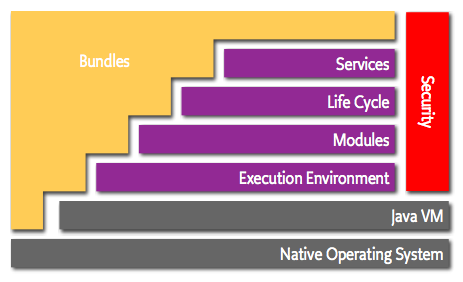
\includegraphics[width=0.7\linewidth]{Bilder/layering-osgi.png}
% 	\captionof{figure}[OSGi Architektur]{OSGi Architektur\footnotemark }
% 	\label{fig:osgi}
% \end{minipage}
% \footnotetext{Quelle: \url{http://www.osgi.org/Technology/WhatIsOSGi}}

% \subsection{Tabellen}
% In diesem Abschnitt wird eine Tabelle (siehe Tabelle \ref{tab:beispiel}) dargestellt.

% \vspace{1em}
% \begin{table}[!h]
% 	\centering
% 	\begin{tabular}{|l|l|l|}
% 		\hline
% 		\textbf{Name} & \textbf{Name} & \textbf{Name}\\
% 		\hline
% 		1 & 2 & 3\\
% 		\hline
% 		4 & 5 & 6\\
% 		\hline
% 		7 & 8 & 9\\
% 		\hline
% 	\end{tabular}
% 	\caption{Beispieltabelle}
% 	\label{tab:beispiel}
% \end{table}

% \pagebreak
% \subsection{Auflistung}
% Für Auflistungen wird die \textit{compactitem}-Umgebung genutzt, wodurch der Zeilenabstand zwischen den Punkten verringert wird.

% \begin{compactitem}
% 	\item Nur
% 	\item ein
% 	\item Beispiel.
% \end{compactitem}

% \subsection{Listings}
% Zuletzt ein Beispiel für ein Listing, in dem Quellcode eingebunden werden kann, siehe Listing \ref{lst:arduino}.

% \vspace{1em}
% \begin{lstlisting}[caption=Arduino Beispielprogramm, label=lst:arduino]
% int ledPin = 13;
% void setup() {
%     pinMode(ledPin, OUTPUT);
% }
% void loop() {
%     digitalWrite(ledPin, HIGH);
%     delay(500);
%     digitalWrite(ledPin, LOW);
%     delay(500);
% }
% \end{lstlisting}

% Die Quellen befinden sich in der Datei \textit{bibo.bib}. Ein Buch- und eine Online-Quelle sind beispielhaft eingefügt. [Vgl. \cite{buch}]

% Abkürzungen lassen sich natürlich auch nutzen (\ac{OSGi}). Weiter oben im Latex-Code findet sich das Verzeichnis.
% \pagebreak

% % ----------------------------------------------------------------------------------------------------------
% % Kapitel
% % ----------------------------------------------------------------------------------------------------------
% \section{Kapitel}
% Lorem ipsum dolor sit amet.

% \subsection{Unterkapitel}
% Lorem ipsum dolor sit amet, consetetur sadipscing elitr, sed diam nonumy eirmod tempor invidunt ut labore et dolore magna aliquyam erat, sed diam voluptua. At vero eos et accusam et justo duo dolores et ea rebum. Stet clita kasd gubergren, no sea takimata sanctus est Lorem ipsum dolor sit amet. Lorem ipsum dolor sit amet, consetetur sadipscing elitr, sed diam nonumy eirmod tempor invidunt ut labore et dolore magna aliquyam erat, sed diam voluptua. At vero eos et accusam et justo duo dolores et ea rebum. Stet clita kasd gubergren, no sea takimata sanctus est Lorem ipsum dolor sit amet.

% \subsection{Unterkapitel}
% Lorem ipsum dolor sit amet, consetetur sadipscing elitr, sed diam nonumy eirmod tempor invidunt ut labore et dolore magna aliquyam erat, sed diam voluptua. At vero eos et accusam et justo duo dolores et ea rebum. Stet clita kasd gubergren, no sea takimata sanctus est Lorem ipsum dolor sit amet. Lorem ipsum dolor sit amet, consetetur sadipscing elitr, sed diam nonumy eirmod tempor invidunt ut labore et dolore magna aliquyam erat, sed diam voluptua. At vero eos et accusam et justo duo dolores et ea rebum. Stet clita kasd gubergren, no sea takimata sanctus est Lorem ipsum dolor sit amet.
% \pagebreak

% % ----------------------------------------------------------------------------------------------------------
% % Kapitel
% % ----------------------------------------------------------------------------------------------------------
% \section{Kapitel}
% Lorem ipsum dolor sit amet.

% \subsection{Unterkapitel}
% Lorem ipsum dolor sit amet, consetetur sadipscing elitr, sed diam nonumy eirmod tempor invidunt ut labore et dolore magna aliquyam erat, sed diam voluptua. At vero eos et accusam et justo duo dolores et ea rebum. Stet clita kasd gubergren, no sea takimata sanctus est Lorem ipsum dolor sit amet. Lorem ipsum dolor sit amet, consetetur sadipscing elitr, sed diam nonumy eirmod tempor invidunt ut labore et dolore magna aliquyam erat, sed diam voluptua. At vero eos et accusam et justo duo dolores et ea rebum. Stet clita kasd gubergren, no sea takimata sanctus est Lorem ipsum dolor sit amet.

% \subsection{Unterkapitel}
% Lorem ipsum dolor sit amet, consetetur sadipscing elitr, sed diam nonumy eirmod tempor invidunt ut labore et dolore magna aliquyam erat, sed diam voluptua. At vero eos et accusam et justo duo dolores et ea rebum. Stet clita kasd gubergren, no sea takimata sanctus est Lorem ipsum dolor sit amet. Lorem ipsum dolor sit amet, consetetur sadipscing elitr, sed diam nonumy eirmod tempor invidunt ut labore et dolore magna aliquyam erat, sed diam voluptua. At vero eos et accusam et justo duo dolores et ea rebum. Stet clita kasd gubergren, no sea takimata sanctus est Lorem ipsum dolor sit amet.
% \pagebreak

% % ----------------------------------------------------------------------------------------------------------
% % Kapitel
% % ----------------------------------------------------------------------------------------------------------
% \section{Kapitel}
% Lorem ipsum dolor sit amet.

% \subsection{Unterkapitel}
% Lorem ipsum dolor sit amet, consetetur sadipscing elitr, sed diam nonumy eirmod tempor invidunt ut labore et dolore magna aliquyam erat, sed diam voluptua. At vero eos et accusam et justo duo dolores et ea rebum. Stet clita kasd gubergren, no sea takimata sanctus est Lorem ipsum dolor sit amet. Lorem ipsum dolor sit amet, consetetur sadipscing elitr, sed diam nonumy eirmod tempor invidunt ut labore et dolore magna aliquyam erat, sed diam voluptua. At vero eos et accusam et justo duo dolores et ea rebum. Stet clita kasd gubergren, no sea takimata sanctus est Lorem ipsum dolor sit amet.

% \subsection{Unterkapitel}
% Lorem ipsum dolor sit amet, consetetur sadipscing elitr, sed diam nonumy eirmod tempor invidunt ut labore et dolore magna aliquyam erat, sed diam voluptua. At vero eos et accusam et justo duo dolores et ea rebum. Stet clita kasd gubergren, no sea takimata sanctus est Lorem ipsum dolor sit amet. Lorem ipsum dolor sit amet, consetetur sadipscing elitr, sed diam nonumy eirmod tempor invidunt ut labore et dolore magna aliquyam erat, sed diam voluptua. At vero eos et accusam et justo duo dolores et ea rebum. Stet clita kasd gubergren, no sea takimata sanctus est Lorem ipsum dolor sit amet.
% \pagebreak

% ----------------------------------------------------------------------------------------------------------
% Literatur
% ----------------------------------------------------------------------------------------------------------
\renewcommand\refname{Quellenverzeichnis}
\bibliographystyle{myalpha}
\bibliography{bibo}
\pagebreak

% % ----------------------------------------------------------------------------------------------------------
% % Anhang
% % ----------------------------------------------------------------------------------------------------------
% \pagenumbering{Roman}
% \setcounter{page}{1}
% \lhead{Anhang \thesection}

% \begin{appendix}
% \section*{Anhang}
% \phantomsection
% \addcontentsline{toc}{section}{Anhang}
% \addtocontents{toc}{\vspace{-0.5em}}

% \section{GUI}
% Ein toller Anhang.

% \subsection*{Screenshot}
% \label{app:screenshot}
% Unterkategorie, die nicht im Inhaltsverzeichnis auftaucht.

% \end{appendix}


% \newpage
% \thispagestyle{empty}
% \begin{center}
% 	\vspace*{5em}
% 	\huge\textbf{Erklärung}\\
% \end{center}
% \vspace{2em}
% Hiermit versichere ich, dass ich meine Abschlussarbeit selbständig verfasst und keine anderen als die angegebenen Quellen und Hilfsmittel benutzt habe.

% \vspace{4em}
% \begin{minipage}{\linewidth}
% 	\begin{tabular}{p{15em}p{15em}}
% 		Datum: &  .......................................................\\
% 		& \centering (Unterschrift)\\
% 	\end{tabular}
% \end{minipage}

\end{document}
